% XeLaTeX can use any Mac OS X font. See the setromanfont command below.
% Input to XeLaTeX is full Unicode, so Unicode characters can be typed directly into the source.

% The next lines tell TeXShop to typeset with xelatex, and to open and save the source with Unicode encoding.

%!TEX TS-program = xelatex
%!TEX encoding = UTF-8 Unicode

\documentclass[11pt,twoside,openany]{book}
\usepackage{multirow}
\usepackage{pdfpages}

\usepackage{xspace}

\usepackage{array}
\usepackage{lipsum}

\usepackage{algorithm}
\usepackage{algpseudocode}

\usepackage{geometry}                % See geometry.pdf to learn the layout options. There are lots.
%\usepackage[margin=1cm]{geometry}


% \addtolength{\textwidth}{1.75in}
%
% \addtolength{\topmargin}{-.875in}
% \addtolength{\textheight}{1.75in}

\geometry{a4paper,left=20mm,top=20mm,bottom=50mm,total={162mm,230mm}}                   % ... or a4paper or a5paper or ...
%\geometry{landscape}                % Activate for for rotated page geometry
%\usepackage[parfill]{parskip}    % Activate to begin paragraphs with an empty line rather than an indent
\usepackage{amssymb}
%\usepackage{todonotes}
\setlength{\marginparwidth}{2cm}
\usepackage[backgroundcolor=white,bordercolor=blue,linecolor=blue,textwidth=1cm]{todonotes}
\usepackage{booktabs}
\usepackage{longtable}
\usepackage{url}

\usepackage[depth=4]{bookmark}


\usepackage{algorithm}
\usepackage{algpseudocode}

\usepackage{imakeidx}
\usepackage[utf8]{inputenc}
\usepackage[T1]{fontenc}
\makeindex[intoc]

\usepackage[font=normalsize]{caption}

\renewcommand{\theparagraph}{\S\arabic{paragraph}}
\setcounter{secnumdepth}{4}


\usepackage{xcolor}
\usepackage{listings}

\makeatletter
\global\let\tikz@ensure@dollar@catcode=\relax
\makeatother

\definecolor{mGreen}{rgb}{0,0.6,0}
\definecolor{mGray}{rgb}{0.5,0.5,0.5}
\definecolor{mPurple}{rgb}{0.58,0,0.82}
\definecolor{backgroundColour}{rgb}{0.95,0.95,0.92}
\definecolor{gray}{rgb}{0.4,0.4,0.4}
\definecolor{darkblue}{rgb}{0.0,0.0,0.6}
\definecolor{cyan}{rgb}{0.0,0.6,0.6}

\lstdefinestyle{CStyle}{
    backgroundcolor=\color{backgroundColour},
    commentstyle=\color{mGreen},
    keywordstyle=\color{magenta},
    numberstyle=\tiny\color{mGray},
    stringstyle=\color{mPurple},
    basicstyle=\scriptsize\ttfamily,
    breakatwhitespace=false,
    breaklines=true,
    captionpos=b,
    keepspaces=true,
    numbers=left,
    numbersep=5pt,
    showspaces=false,
    showstringspaces=false,
    showtabs=false,
    tabsize=2,
    language=C
}


\lstset{
  backgroundcolor=\color{white},   % choose the background color; you must add \usepackage{color} or \usepackage{xcolor}; should come as last argument
  basicstyle=\footnotesize\ttfamily,        % the size of the fonts that are used for the code
  breakatwhitespace=false,         % sets if automatic breaks should only happen at whitespace
  breaklines=true,                 % sets automatic line breaking
  captionpos=b,                    % sets the caption-position to bottom
  commentstyle=\color{gray},    % comment style
  deletekeywords={...},            % if you want to delete keywords from the given language
  %escapeinside={\%*}{*)},          % if you want to add LaTeX within your code
  %extendedchars=true,              % lets you use non-ASCII characters; for 8-bits encodings only, does not work with UTF-8
  %firstnumber=1000,                % start line enumeration with line 1000
  frame=single,                    % adds a frame around the code
  keepspaces=true,                 % keeps spaces in text, useful for keeping indentation of code (possibly needs columns=flexible)
  keywordstyle=\color{blue},       % keyword style
  language=C,                 % the language of the code
  %morekeywords={*,...},            % if you want to add more keywords to the set
  numbers=left,                    % where to put the line-numbers; possible values are (none, left, right)
  numbersep=5pt,                   % how far the line-numbers are from the code
  numberstyle=\tiny\color{gray}, % the style that is used for the line-numbers
  rulecolor=\color{black},         % if not set, the frame-color may be changed on line-breaks within not-black text (e.g. comments (green here))
  showspaces=false,                % show spaces everywhere adding particular underscores; it overrides 'showstringspaces'
  showstringspaces=false,          % underline spaces within strings only
  showtabs=false,                  % show tabs within strings adding particular underscores
  stepnumber=1,                    % the step between two line-numbers. If it's 1, each line will be numbered
  stringstyle=\color{black},     % string literal style
  tabsize=2,                     % sets default tabsize to 2 spaces
}

\lstset{
  columns=fullflexible,
  showstringspaces=false,
  commentstyle=\color{gray}\upshape,
  backgroundcolor=\color{backgroundColour},
  commentstyle=\color{mGreen},
  keywordstyle=\color{magenta},
  numberstyle=\tiny\color{mGray},
  stringstyle=\color{mPurple},
  basicstyle=\scriptsize\ttfamily,
  tabsize=2
}

\lstdefinelanguage{XML}
{
  morestring=[b]",
  morestring=[s]{>}{<},
  morecomment=[s]{<?}{?>},
  stringstyle=\color{black},
  identifierstyle=\color{darkblue},
  keywordstyle=\color{cyan},
  morekeywords={xmlns,version,type}% list your attributes here
}


% Will Robertson's fontspec.sty can be used to simplify font choices.
% To experiment, open /Applications/Font Book to examine the fonts provided on Mac OS X,
% and change "Hoefler Text" to any of these choices.

\usepackage{fontspec,xltxtra,xunicode}
\defaultfontfeatures{Mapping=tex-text}
\setromanfont[Mapping=tex-text]{Optima}
\setsansfont[Scale=MatchLowercase,Mapping=tex-text]{Optima}
\setmonofont[Scale=MatchLowercase]{Andale Mono}

%%%% Graphics
\usepackage{graphicx}
\usepackage{tikz}
\definecolor{unilublue}{RGB}{55,149,218}
\definecolor{sntred}{RGB}{219,46,27}
\definecolor{sntpurple}{RGB}{86,30,130}
%\definecolor{sntblue}{RGB}{50,130,207}
\definecolor{sntblue}{RGB}{55,149,218}

\pgfdeclareimage[width=30mm]{logo-snt}{logos/logo-snt}
\pgfdeclareimage[width=30mm]{logo-uni-lu}{logos/logo-uni-lu}

%%%% Fancy
\usepackage{fancyhdr}

%%%% Increase page length
\addtolength{\textheight}{1in}

%%%% Sections
\usepackage{sectsty}
\allsectionsfont{\sffamily}

\setlength{\parskip}{1em}

%\renewcommand{\,}{$^{\cdot}$}

\usepackage{hyperref}
\hypersetup{
    colorlinks,
    citecolor=black,
    filecolor=black,
    linkcolor=black,
    urlcolor=black
}


%%%% Title
\newcommand{\titleone}{\textsf{FAQAS Framework}}
\newcommand{\titletwo}{\textsf{SUTP}}
\newcommand{\titlethree}{\textsf{Software Unit Test Plan}}

\newcommand{\todoinline}[1]{\todo[color=orange,inline]{ \textbf{TODO}: #1 }}

\newcommand{\TODO}[1]{\todo[color=orange,inline]{ \textbf{TODO}: #1 }}
\newcommand{\OSCAR}[1]{\todo[color=yellow,inline]{ \textbf{OSCAR}: #1 }}
\newcommand{\DONE}[1]{\todo[color=green,inline]{ \textbf{DONE}: #1 }}

\newcommand{\CHANGEDTWO}[1]{\textcolor{black}{#1}}

\newcommand{\EMPH}[1]{\textbf{\emph{#1}}}
\newcommand{\INDEX}[1]{\index{\MakeLowercase{#1}}\EMPH{#1}}

\newcommand{\MASS}{\textit{MASS}\xspace}

\newcounter{paranum}
\newcommand{\RQ}{\vspace{10pt}\noindent\textbf{FAQAS-SSS-REQ-\refstepcounter{paranum}\ifnum\value{paranum}<10 00\else 0\fi\theparanum}\textbf}

\newcommand{\remark}{\textbf{Remark:}\xspace}

\begin{document}

\pagestyle{fancy}
\renewcommand{\sectionmark}[1]{\markright{\textit{#1}}}

\renewcommand{\headrulewidth}{2pt}% 2pt header rule
\renewcommand{\headrule}{\hbox to\headwidth{%
  \color{sntblue}\leaders\hrule height \headrulewidth\hfill}}

\fancyhf{}

%\lhead{\fancyplain{}{\setlength{\unitlength}{1mm}
%\begin{picture}(0,0)
%\put(0,-4){
\includegraphics[width=50pt]{logos/logo-snt}}
%\end{picture}}}

\lhead{\fancyplain{}{\textit{}}}

\rhead{\fancyplain{}{\rightmark }}

\fancyfoot[C]{%
\begin{tikzpicture}[remember picture,overlay]
\path [fill=sntred]    ([xshift=88pt,yshift=20pt]current page.south west) rectangle
                       ([xshift=229pt,yshift=50pt] current page.south west);
\path [fill=sntpurple] ([xshift=229pt,yshift=20pt] current page.south west) rectangle
                       ([xshift=370pt,yshift=50pt] current page.south west);
\path [fill=sntblue]   ([xshift=370pt,yshift=20pt] current page.south west) rectangle
                       ([xshift=510pt,yshift=50pt] current page.south west);
\end{tikzpicture}
}

\fancyfoot[RO]{
\begin{tikzpicture}[remember picture,overlay]
\node [circle, ultra thick, fill=white, draw=sntblue] at ([xshift=530pt,yshift=35pt] current page.south west) {\thepage};
\end{tikzpicture}}

\fancyfoot[LE]{
\begin{tikzpicture}[remember picture,overlay]
\node [circle, ultra thick, fill=white, draw=sntblue] at ([xshift=65pt,yshift=35pt] current page.south west) {\thepage};
\end{tikzpicture}}


\newcommand{\CHANGED}[1]{\textcolor{blue}{#1}}
\newcommand{\prog}{P}
\newcommand{\prop}{}

\newcommand{\FAQAS}{FAQAS-framework\xspace}

\newcommand{\REVISION}[2]{\todo{\tiny{#1}}\color{blue}{#2}\color{black}}

\newcommand{\REVTWO}[2]{#2}

\thispagestyle{empty}

\begin{tikzpicture}[remember picture,overlay]
\path [fill=sntred]    ([xshift=30pt,yshift=20pt]current page.south west) rectangle
                       ([xshift=210pt,yshift=50pt] current page.south west);
\path [fill=sntpurple] ([xshift=210pt,yshift=20pt] current page.south west) rectangle
                       ([xshift=390pt,yshift=50pt] current page.south west);
\path [fill=sntblue]   ([xshift=390pt,yshift=20pt] current page.south west) rectangle
                       ([xshift=570pt,yshift=51pt] current page.south west);
\path [fill=unilublue] ([xshift=30pt,yshift= 50pt] current page.south west) --
                       ([xshift=570pt,yshift= 50pt] current page.south west)
                       [rounded corners=20pt] --
                       ([xshift=570pt,yshift=740pt] current page.south west)
                       [sharp corners] --
                       ([xshift=30pt,yshift=740pt] current page.south west);
\node [fill=white,rounded corners=0pt,inner xsep=6pt,inner ysep=3pt]
      at ([xshift=523pt,yshift=120pt] current page.south west)
      {\pgfuseimage{logo-uni-lu}};

\node [fill=white,rounded corners=2pt,inner xsep=6pt,inner ysep=3pt]
      at ([xshift=520pt,yshift=780pt] current page.south west)
      {\pgfuseimage{logo-snt}};

%\node [circle, fill=white, draw=sntblue] at ([xshift=550pt,yshift=35pt] current page.south west) {a};

\node[draw=none,fill=none,right] at (-1, -7){\color{white}\LARGE\bf\titleone};
\node[draw=none,fill=none,right] at (-1, -8){\color{white}\LARGE\bf\titletwo};
\node[draw=none,fill=none,right] at (-1, -9){\color{white}\LARGE\bf\titlethree};

\node[draw=none,fill=none,right] at (-1, -12){\color{white}\Large\textsf{O. Cornejo, F. Pastore, E. Viganò}};
\node[draw=none,fill=none,right] at (-1, -13){\color{white}\Large\textsf{Interdisciplinary Centre for Security, Reliability and Trust}};
\node[draw=none,fill=none,right] at (-1, -14){\color{white}\Large\textsf{University of Luxembourg}};
\node[draw=none,fill=none,right] at (11, -16){\color{white}\textsf{ITT-1-9873-ESA-FAQAS-SUTP}};
\node[draw=none,fill=none,right] at (11, -17){\color{white}\Large\textsf{Issue 4, Rev. 1}};
\node[draw=none,fill=none,right] at (11, -18){\color{white}\Large\textsf{\today}};
\node[draw=none,fill=none,right] at (-1, -24){\color{white}\tiny\textsf{EUROPEAN SPACE AGENCY. CONTRACT REPORT.}};
\node[draw=none,fill=none,right] at (-1, -24.3){\color{white}\tiny\textsf{The work described in this report was done under ESA contract. Responsibility for the contents resides in the author or organisation that prepared it.}};
\node[draw=none,fill=none,right] at (-1, -24.8){\color{white}\tiny\textsf{The copyright in this document is vested in the University of Luxembourg.}};
\node[draw=none,fill=none,right] at (-1, -25.1){\color{white}\tiny\textsf{This document may only be reproduced in whole or in part, or stored in a retrieval system,or transmitted in any form, or by any means electronic,}};
\node[draw=none,fill=none,right] at (-1, -25.4){\color{white}\tiny\textsf{mechanical, photocopying or otherwise, either with the prior permission of the University of Luxembourg or in accordance with the terms of ESTEC Contract No. 4000128969/19/NL/AS.}};

\node[draw=none,fill=none,right] at (-1, -24){\color{white}\tiny\textsf{EUROPEAN SPACE AGENCY. CONTRACT REPORT.}}; 
\node[draw=none,fill=none,right] at (-1, -24.3){\color{white}\tiny\textsf{The work described in this report was done under ESA contract. Responsibility for the contents resides in the author or organisation that prepared it.}};
\node[draw=none,fill=none,right] at (-1, -24.8){\color{white}\tiny\textsf{The copyright in this document is vested in the University of Luxembourg.}};
\node[draw=none,fill=none,right] at (-1, -25.1){\color{white}\tiny\textsf{This document may only be reproduced in whole or in part, or stored in a retrieval system,or transmitted in any form, or by any means electronic,}}; 
\node[draw=none,fill=none,right] at (-1, -25.4){\color{white}\tiny\textsf{mechanical, photocopying or otherwise, either with the prior permission of the University of Luxembourg or in accordance with the terms of ESTEC Contract No. 4000128969/19/NL/AS.}};


\end{tikzpicture}

\newpage


% !TEX root = MAIN.tex

\section*{Revisions}
\label{sec:revisions}


\setlength\LTleft{0pt}
\setlength\LTright{0pt}
\tiny 
%@{\extracolsep{\fill}}
\begin{longtable}{|p{2cm}|p{1cm}|p{1.5cm}|p{9cm}|@{}}
\label{table:codeoperators} \\
\hline
\textbf{Issue Number}&\textbf{Date}&\textbf{Authors}&\textbf{Description}\\
\hline
ITT-1-9873-ESA-FAQAS-FR
Issue 1 Rev. 1&
October 29th, 2021&
Fabrizio Pastore, Oscar Cornejo, Enrico Viganò&
\begin{minipage}{8cm}
Initial release.
\end{minipage}
\\
\hline
ITT-1-9873-ESA-FAQAS-FR
Issue 1 Rev. 2&
November 11th, 2021&
Fabrizio Pastore, Oscar Cornejo, Enrico Viganò&
\begin{minipage}{8cm}
Added Chapter~\ref{chap:deliverables_summary} (deliverables summary).\\
Added Chapter~\ref{ch:toolset} (description of toolset package).\\
Added information about input and outputs of the tools in Chapter~\ref{chapter:methodology} (see blue text).
\end{minipage}
\\
\hline
                                                    
\end{longtable}
\normalsize

\clearpage


\tableofcontents


% !TEX root = MAIN.tex

\chapter{Scope and content}

This document is the deliverable SSS of the ESA activity ITT-1-9873-ESA. It concerns requirements specification for the \emph{FAQAS framework} to be delivered by ITT-1-9873-ESA. Following the structure described in the SoW \emph{AO9873-ws00pe\_SOW.pdf}, it provides the structured requirements baseline for the FAQAS framework according to ECSS-E-ST-40C Annex B.
 
\section{Applicable and reference documents}

\begin{itemize}
\item{D1 - Mutation testing survey}
\item{D2 - Study of mutation testing applicability to space software}
\end{itemize}

\chapter{Terms, definitions and abbreviated terms}

\begin{itemize}
\item{FAQAS}: activity ITT-1-9873-ESA
\item{FAQAS-framework}: software system to be released at the end of WP4 of FAQAS
\item{D2}: Deliverable D2 of FAQAS, \emph{Study of mutation testing applicability to space software}
\item{KLEE}: Third party test generation tool, details are provided in D2.
\item{SUT}: Software under test, i.e, the software that should be mutated by means of mutation testing.
\item{WP}: Work package
\end{itemize}

\clearpage
 



% !TEX root = MAIN.tex

\chapter{Software Release Overview}

\chapter{Status of the Software Configuration Item}

% !TEX root = MAIN.tex

\chapter{Software Unit Testing and Software Integration Testing}

\section{Organization}

The unit tests are to be prepared by SnT in the form of Bash shell scripts. Testing will be conducted by SnT personnel.

If any software problems occur during testing a development issue shall be raised in GitLab Issue Tracker, which shall be amended by SnT personnel.

%\section{Master schedule}


\section{Resource Summary}

Unit tests make use of the \FAQAS. Tests will be performed in one hardware platform, a x86-64 desktop PC. Unit test execution time should not exceed one day for all target platforms combined.

\section{Responsibilities}

The unit tests are to be prepared by SnT personnel.

The tests will be conducted by a SnT specialist who will also have the responsibility of reporting any occurring software issues.

\section{Tool, techniques and methods}

Unit tests are specified in Bash files. Each unit test contains a launcher script that configures the environment for the correct execution of \FAQAS, and a source code example for its mutation. The launcher script will invoke a dedicated operator Bash script, that generates the corresponding mutants and assesses its results.

\section{Personnel and Personnel Training Requirements}

Unit testing can be performed by a single person using a general script. No special training is needed.

\section{Risks and Contingencies}

The unit testing campaign does not have any risk.

% !TEX root = MAIN.tex

\chapter{Control procedure for Software Unit Testing}
\label{chapter:control:procedure}

Technical and organizational problems shall be reported on in GitLab Issue Tracker for the FAQAS-framework, which is available at https://gitlab.uni.lu/fpastore/FAQAS.
The FAQAS management will take care of conflict resolution.


% !TEX root =  ../Main.tex
\subsection{Space Software Mutation Testing Process}
\label{sec:approach}

\begin{figure}[h!]
\begin{center}
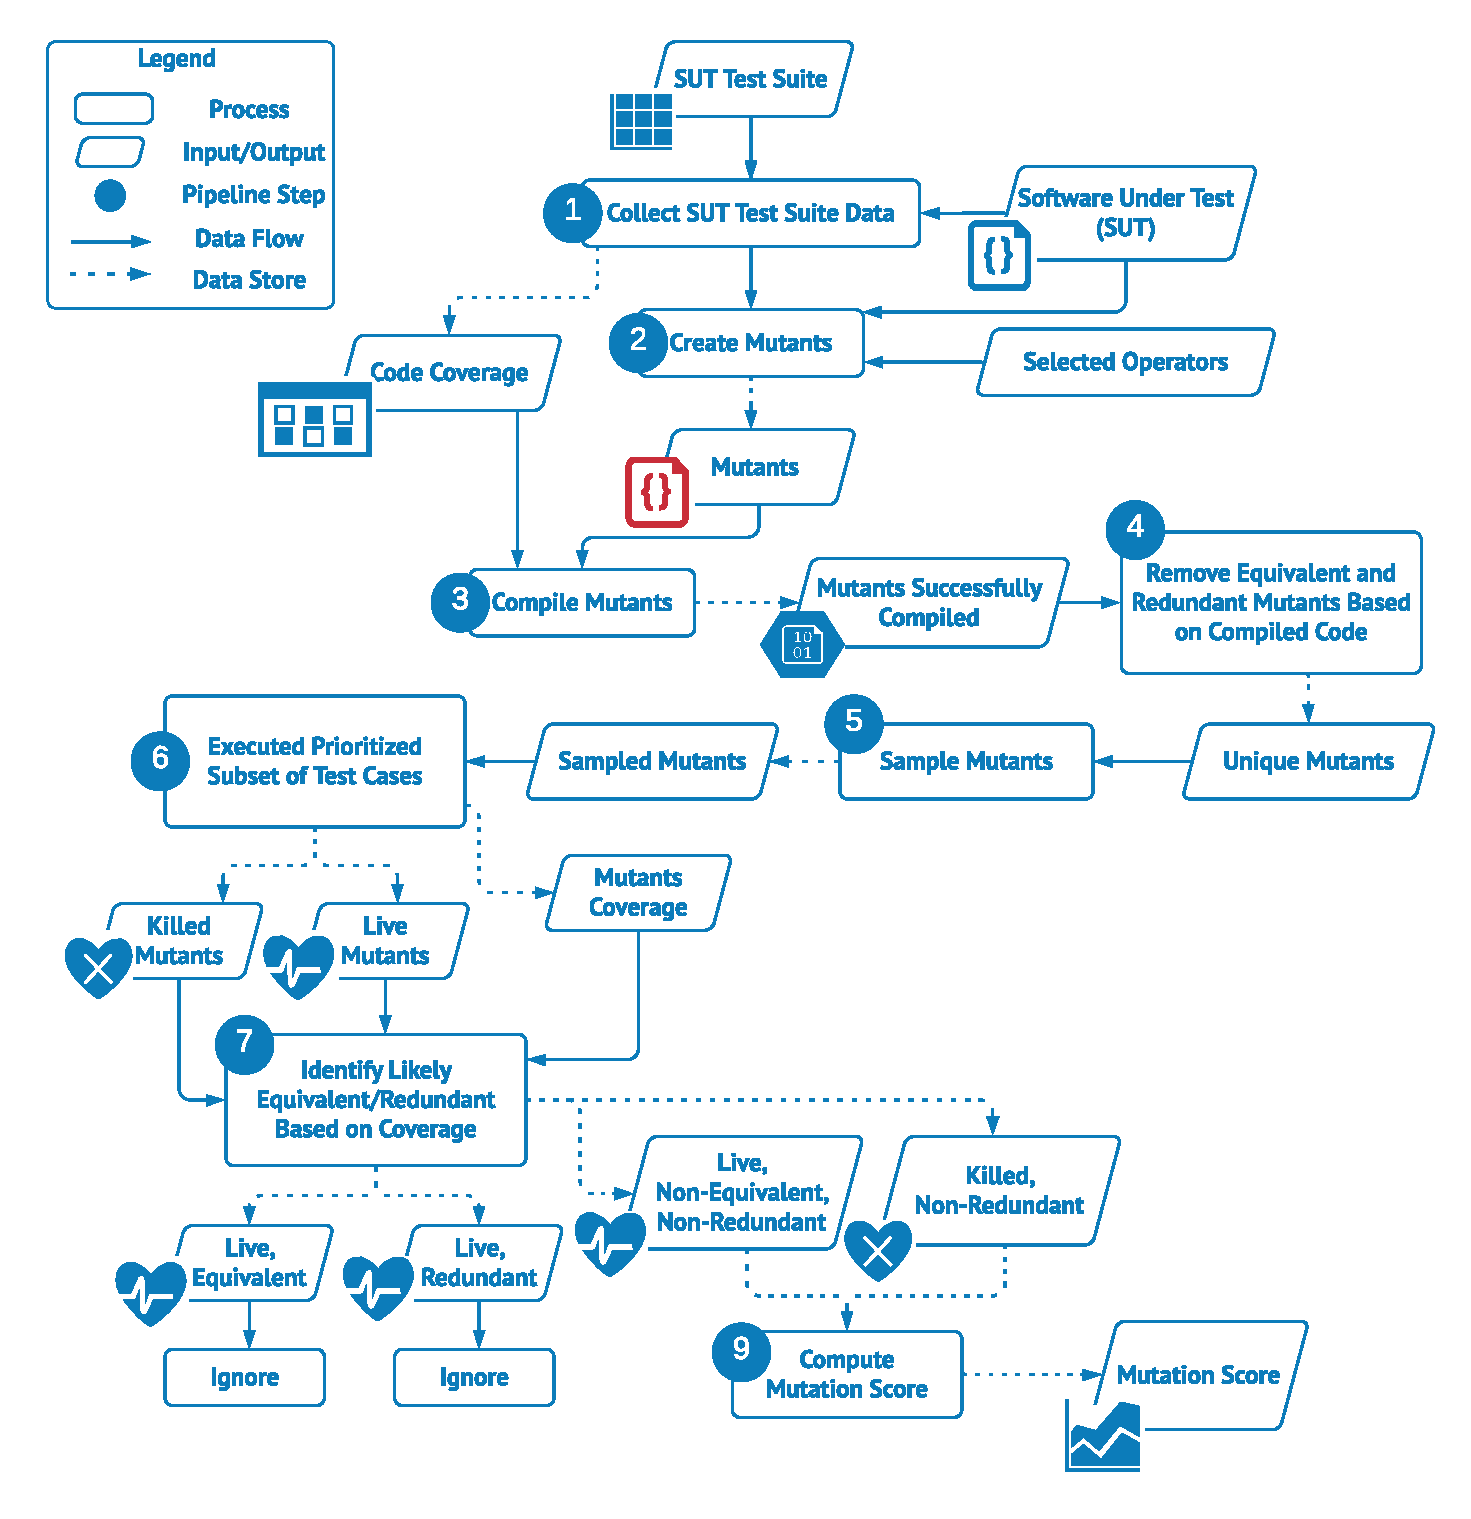
\includegraphics[width=\textwidth]{images/MT}
\caption{Overview of the proposed Mutation Testing Pipeline}
\label{fig:approach}
\end{center}
\end{figure}

Figure~\ref{fig:approach} provides an overview of the mutation testing process that we propose, namely Scalable Mutation Testing for Space Software  (\APPR). We describe each step in the following paragraphs. 

\subsubsection{Step 1}

In Step 1, the test suite is executed against the software under test (SUT) and code coverage information is collected. 
More precisely, we rely state-of-the art code coverage tools such as gcov~\cite{GCOV} and Vector CAST~\cite{VectorCAST} 
to record the number of times each line of code of the SUT has been exercised by a test case.

\subsubsection{Step 2}

In Step 2, we automatically generate mutants for the SUT by relying on a set of selected mutation operators.
In \APPR, based on the considerations provided in Section~\ref{sec:related:operators}, we rely on an extended sufficient set of mutation operators, which are listed in Table~\ref{table:sufficient_operators}.
In addition, in our experiments, we evaluate the feasibility of relying only on the SDL operators instead of the whole sufficient set of operators.

% !TEX root =  ../Main.tex

\newcommand{\op}{\mathit{op}}
\newcommand{\ArithmeticSet}{ \texttt{+}, \texttt{-}, \texttt{*}, \texttt{/}, \texttt{\%} }
\newcommand{\LogicalSet}{ \texttt{&&}, \texttt{||} }
\newcommand{\RelationalSet}{ \texttt{>}, \texttt{>=}, \texttt{<}, \texttt{<=}, \texttt{==}, \texttt{!=} }
\newcommand{\BitWiseSet}{ \texttt{\&}, \texttt{|}, \land }
\newcommand{\ShiftSet}{ \texttt{>>}, \texttt{<<} }


\begin{table}[h]
\caption{Implemented set of mutation operators.}
\label{table:operators} 
\centering
\scriptsize
\begin{tabular}{|@{}p{4mm}@{}|@{}p{2cm}@{\hspace{1pt}}|@{}p{11.1cm}@{}|}
\hline
&\textbf{Operator} & \textbf{Description$^{*}$} \\
\hline
\multirow{7}{*}{\rotatebox{90}{\emph{Sufficient Set}}}&ABS               & $\{(v, -v)\}$	\\
\cline{2-3}
&AOR               & $\{(\op_1, op_2) \,|\, \op_1, \op_2 \in \{ \ArithmeticSet \} \land \op_1 \neq \op_2 \} $       \\
&    			  & $\{(\op_1, \op_2) \,|\, \op_1, \op_2 \in \{\texttt{+=}, \texttt{-=}, \texttt{*=}, \texttt{/=}, \texttt{\%} \texttt{=}\} \land \op_1 \neq \op_2 \} $       \\
\cline{2-3}
&ICR               & $\{i, x) \,|\, x \in \{1, -1, 0, i + 1, i - 1, -i\}\}$           \\
\cline{2-3}
&LCR               & $\{(\op_1, \op_2) \,|\, \op_1, \op_2 \in \{ \texttt{\&\&}, || \} \land \op_1 \neq \op_2 \}$            \\
&				  & $\{(\op_1, \op_2) \,|\, \op_1, \op_2 \in \{ \texttt{\&=}, \texttt{|=}, \texttt{\&=}\} \land \op_1 \neq \op_2 \}$            \\
&				  & $\{(\op_1, \op_2) \,|\, \op_1, \op_2 \in \{ \texttt{\&}, \texttt{|}, \texttt{\&\&}\} \land \op_1 \neq \op_2 \}$            \\
\cline{2-3}
&ROR               & $\{(\op_1, \op_2) \,|\, \op_1, \op_2 \in \{ \RelationalSet \}\}$            \\
&				  & $\{ (e, !(e)) \,|\, e \in \{\texttt{if(e)}, \texttt{while(e)}\} \}$ \\
\cline{2-3}
&SDL               & $\{(s, \texttt{remove}(s))\}$            \\
\cline{2-3}
&UOI               & $\{ (v, \texttt{--}v), (v, v\texttt{--}), (v, \texttt{++}v), (v, v\texttt{++}) \}$            \\   
\hline
\hline
\multirow{5}{*}{\rotatebox{90}{\emph{OODL}}}&AOD               & $\{((t_1\,op\,t_2), t_1), ((t_1\,op\,t_2), t_2) \,|\, op \in \{ \ArithmeticSet \} $       \\ 
\cline{2-3}
&LOD               & $\{((t_1\,op\,t_2), t_1), ((t_1\,op\,t_2), t_2) \,|\, op \in \{  \} \}$       \\ 
\cline{2-3}
&ROD               & $\{((t_1\,op\,t_2), t_1), ((t_1\,op\,t_2), t_2) \,|\, op \in \{ \RelationalSet \} \}$       \\ 
\cline{2-3}
&BOD               & $\{((t_1\,op\,t_2), t_1), ((t_1\,op\,t_2), t_2) \,|\, op \in \{ \BitWiseSet \} \}$       \\ 
\cline{2-3}
&SOD               & $\{((t_1\,op\,t_2), t_1), ((t_1\,op\,t_2), t_2) \,|\, op \in \{ \ShiftSet \} \}$       \\ 
%\hline
%COR               & $\{(\op_1, \op_2) \,|\, \op_1, \op_2 \in \{ \texttt{\&\&}, \texttt{||}, \land \} \land \op_1 \neq \op_2 \}$            \\
\hline
\hline
\multirow{3}{*}{\rotatebox{90}{\emph{Other}}}&LVR			& $\{(l_1, l_2) \,|\, (l_1, l_2) \in \{(0,-1), (l_1,-l_1), (l_1, 0), (\mathit{true}, \mathit{false}), (\mathit{false}, \mathit{true})\}\}$\\
&&\\
&&\\
\hline
\end{tabular}

$^{*}$Each pair in parenthesis shows how a program element is modified by the mutation operator. Th eleft element of the pair is replaced with the right element. We follow standard syntax~\cite{kintis2018effective}. Program elements are literals ($l$), integer literals ($i$), boolean expressions ($e$), operators ($\op$), statements ($s$), variables ($v$), and terms ( $t_i$, which might be either variables or literals).
\end{table}

To automatically generate mutants, we have extended SRCIRor~\cite{hariri2018srciror} to include all the mutation operators of the sufficient set. After mutating the original source file, our extension saves the mutated source file and keeps track of the mutation applied. 

\subsubsection{Step 3}
\label{codeDriven:stepThree}

In Step 3, we compile mutants by relying on the build system of the SUT. To this end, we have developed a toolset that, for each mutated source file: (1) backs-up the original source file, (2) renames the mutated source file as the original source file, (3) runs the build system (e.g., executes the command \texttt{make}), (4) copies the generated executable mutant in a dedicated folder, (5) restores the original source file. 

Build systems create one object file for each source file to be compiled and then link these object files together into the final executable. For this reason, since we modify at most two source files for each mutant (i.e., the mutated file and the file restored from previous mutation), we can reuse almost all the compiled object files in subsequent compilation runs, thus speeding up the compilation of multiple mutants. Some preliminary experiments conducted with our case study systems have shown that additional compile-time optimizations (e.g., mutant schemata) are not necessary to make the compilation of mutants feasible.

\MREVISION{C-P-24}{Mutants that lead to compilation errors are discarded. Concerning compilation warnings, we assume the build system of the SUT has been properly configured; more precisely, if the system should compile without warnings, the compiler is expected to be configured to treat warnings as errors otherwise mutants that lead to warning are retained.}

\subsubsection{Step 4}

In Step 4, we rely on trivial compiler optimizations to identify and remove equivalent and redundant mutants. 
\MREVISION{C-P-15}{We aim to enable all the available optimizations (e.g., \texttt{-O3} or \texttt{-Ofast} in GCC).}
If the SUT is already configured to be compiled with optimizations enabled, Step 4 consists of first computing the SHA-512 hash summary of all the mutant and original executables and then compare all the generated hash summaries. Hash comparison enables us to (1) determine the presence of equivalent mutants (i.e., mutants having the same hash of the original executable), and (2) identify duplicate mutants (i.e., mutants with the same hash). %Mutants that are identified as being either equivalent and redundant mutants are ignored in the following steps of \APPR. 
Equivalent and redundant mutants are discarded.
The outcome of Step 4 is a set of \emph{unique mutants}, i.e., mutants with compiled code that differs from the original software and any other mutant.

If the SUT should not be compiled with compiler optimizations enabled, we identify equivalent and redundant mutants by re-executing Step 3 with compiler optimizations enabled and then apply Step 4.
%The executables generated by this additional run of Step 3 are used only to identify equivalent mutants, not to evaluate the SUT test suite, which is based on executables compiled without optimizations (otherwise test cases may fail).

\subsubsection{Step 5}

In Step 5, we sample the mutants to be executed to compute the mutation score. This optimization is based on the results of Zhang et al.~\cite{zhang2013operator}, who compare eight strategies for sampling mutants. In our work, we consider two strategies. The first is the \emph{baseline sampling} strategy, which consists of randomly selecting $r\%$ mutants from the complete mutants set. The second is the \emph{method-based sampling} strategy, which is the best performing strategy in \cite{zhang2013operator} and consists of sampling mutants evenly across all functions of the SUT, i.e., sampling $r\%$ mutants from each set of mutants generated inside a same function.

%In Section~\ref{}, we evaluate which of these sampling strategies lead to mutation score


\subsubsection{Step 6}

In Step 6, we execute a prioritized subset of test cases. 
We execute test cases in sequence, and we select only the ones that satisfy 
the reachability condition (i.e., cover the mutated statement).
Similarly to the approach of Zhang et al. \cite{zhang2013faster}, we define the order of execution of test cases based on their likelihood of killing a mutant. However, we redefined the criteria for the selection of test cases because of the inapplicability of the ones proposed by Zhang et al. (see Section~\ref{sec:scalability}).


\MREVISION{C-P-46}{We execute only covered statements assuming that the test suite is optimal with respect to code coverage. More precisely, we addume that if a statement is not covered there is a good reason for it (e.g., it depends on hardware). 
If a statement is not covered by the test suite, there is no chance that a mutant generated in the non-covered statement can be possibly detected by any test case. 
If the test suite does not reach the required coverage there is no reason to perform mutation testing, because is already known that the test suite is not good.}
%\EMPH{When computing the mutation score, is it fare to not count those not-covered lines?}
%Yes, is it fare because mutation testing assess the quality of existing test suites, and considering non-covered statements would be out of the scope of the technique. Also, including non-covered statements into the mutation score, would not let us to assess correctly the quality of the existing test suite.
%\EMPH{Maybe the approach would be to run the test augmentation process to provide test cases for the missing statements?}
%Yes, the same tools used for test augmentation can be used. We can run them. The main difference is that oracles  for the generated test cases should be manually specified (in the case of test augmentation we may derive the oracle based on the values generated by KLEE/CBMC). However, the evaluation of these generated test suites through mutation testing address a different research question than the one of the project; i.e., we would evaluate test automation tools instead of manual test suites.




%However, we notice that such optimization may not be sufficient when test suites are particularly large; indeed, prioritizing test cases may not be sufficient to reduce execution time. For example, live mutants may lead to the execution of a large number of test cases when almost all the test cases of the test suite exercise the mutated statement. 


To reduce the number of test cases to be executed with a mutant, 
we should first execute the ones that more likely satisfy the necessity condition. 
More precisely, the next test case to be executed in a sequence should be the one that exercises the mutated statement with variable values not observed before. 
Unfortunately, in our context, the size of the SUT and its real-time constraints prevent us from recording all the variable values processed during testing. 

To determine if two test case executions exercise the mutated statement with diverse variable values, we rely on code coverage.
% as a surrogate indicator of  variable values diversity.
%diversity in values assigned to the variables used in a statement. 
Indeed, a difference in the set of instructions being covered by two test cases that exercise the mutated statement may depend on the values used in the mutated statement. 
However, since the behaviour of the whole software depends on all the executed software instructions, we reduce the scope of our code coverage analysis 
%to the file containing the source code of the mutated function. 
to the mutated function, its callers, and its callees.
%to maximize the chances that a change in the behaviour of the software depends on the values used in a mutated statement, we determine that two executions likely exercise a mutated statement with diverse values by focussing on the coverage of 
%the mutated function, its callers, and its callees.
A reduced scope is effective in determining behavioural differences based on the analysis of variable valuations~\cite{Pastore:VART:2014}.

%Since related work focuses on either statement coverage or the frequency of execution of a statement, 
Following related work, we have identified two possible criteria to characterize test case executions based on code coverage:
\begin{itemize}
\item[C1] Identify the set $C_t$ of source code statements being covered by the test case.
%\item[C2] Identify the set of unique pairs $\langle\mathit{statement},\mathit{arity}\rangle$, where $\mathit{statement}$ is a unique identifier for the source code statement, and $\mathit{arity}$ is a symbol (i.e., $1$ or $*$) indicating if the statement has been covered one or more times.
\item[C2] Derive a vector whose values capture the number of times each monitored statement had been covered.
\end{itemize}

We have identified distance metrics that determine how dissimilar two test cases are, and, consequently how likely they exercise the mutated statement with different values. In the case of C1 we rely on the Jaccard and Ochiai index, which are two similarity indexes for binary data successfully used to compare program executions based on code coverage~\cite{Zou:Ochiai:2019,Keller:Jaccard:2017,Briand:2019}. Given two test cases $T_A$ and $T_B$, the Jaccard  ($D_J$) and the Ochiai ($D_O$) distance are computed as follows:

$D_J(T_a,T_b)=\frac{|C_a \cap C_b|}{|C_a \cup C_b|}$ \hspace{5mm} $D_O(T_a,T_b)=1-\frac{|C_a \cap C_b|}{\sqrt{|C_a| * |C_b|}}$, 
$C_a$ and $C_b$ are the set of coverage items exercised by the test cases $T_a$ and $T_b$, respectively.

In the case of C2, we compute the distance between two test cases by relying on the euclidean distance ($D_E$) and the cosine similarity distance ($D_C$), two popular distance metrics used in machine learning. Given two vectors $V_A$ and $V_B$ that capture the number of times each statement has been covered by test cases $T_A$ and $T_B$, the distances $D_E$ and $D_C$ can be computed as follows:

$D_E=\sqrt{\sum_{i=1}^{n}(A_i-B_i)^2}$ 
$D_C= \frac{\sum_{i=1}^{n}A_i*B_i}{\sqrt{\sum_{i=1}^{n}{A_i}^2}*\sqrt{\sum_{i=1}^{n}{B_i}^2}}$,
%Their main difference is that cosine similarity is used when the magnitude of the vectors should not matter.
$A_i$ and $B_i$ refer to the number of times the i-th statement had been covered by test cases $T_A$ and $T_B$, respectively.

Figure~\ref{alg:prioritize} shows the pseudocode of our algorithm for selecting and prioritizing test cases. It generates as output
a prioritized test suite (i.e., \emph{PTS}) that consists of a subset of the test cases that exercise the mutated statement (Line~\ref{alg:prioritize:select}).
Based on the findings of Zhang et al. \cite{zhang2013faster}, we first select the test case that exercises the mutated statement more times (Line~\ref{alg:prioritize:first}) \MREVISION{C-P-17}{ and add it to the prioritized test suite (Line~\ref{alg:prioritize:add}).}
Then, the next selected test case is the one with the largest distance from the closest test case belonging to the set of test cases already selected (Lines~\ref{alg:prioritize:selectStart} to~\ref{alg:prioritize:selectEnd}). 
%is most different than any other test case already included in the prioritized test suite.

%Then, since we aim to maximize test cases diversity, the next selected test case should be the one that is most different than any other test case already included in the prioritized test suite.
%For this reason, for each test case $n$ not selected yet (Line~\ref{alg:prioritize:notSel}), we identify the test case $t$ showing the most similar coverage (i.e., the one with the minimal distance $d$, Line~\ref{alg:prioritize:minD}). We then select the test case $n$ with the highest distance from its closest test case (Lines~\ref{alg:prioritize:selectStart} to~\ref{alg:prioritize:selectEnd}). 

The algorithm iterates as long as it identifies a test case that exercises 
the program instructions differently than the test cases already selected (Line~\ref{alg:prioritize:until}).

Test cases are then executed in the selected order. During the execution we collect code coverage information and identify killed and live mutants.

% !TEX root =  ../Main.tex

\newcommand{\INDA}{10}
\newcommand{\INDB}{15}
\newcommand{\INDC}{5}

%\vspace{-3mm}
\begin{figure}[tb]

\begin{algorithmic}[1]

%\footnotesize
\scriptsize
\Require \emph{TS}, the test suite of the software under test
\Require \emph{Cov}, coverage information, for each test case
\Require \emph{ms}, the mutated statement
\Ensure \emph{PTS}, a list of test cases to be executed, sorted by priority
% (source inputs, follow-up inputs, output data).

\State $\mathit{TS}_m \gets$ subset of $\mathit{TS}$ that cover the mutated statement $\mathit{ms}$, based on \emph{Cov} \label{alg:prioritize:select}
\State $\mathit{PTS} \gets \mathit{new} \mathit{list}$ \textcolor{darkgray}{//this list is initially empty}
\State $\mathit{PTS} \gets$ based on \emph{Cov} select from $\mathit{TS_m}$ the test case $t$ that exercises $\mathit{ms}$ more times \label{alg:prioritize:first}
\State $\mathit{PTS} \gets \mathit{PTS} \cup t$ \textcolor{darkgray}{//include first the test case selected above}  \label{alg:prioritize:add}

\State \textbf{repeat} \label{alg:prioritize:repeat}
\State \hspace{\INDC mm} \textbf{for each} $n$ in the set ($\mathit{TS}_m$ - $\mathit{PTS}$) \textcolor{darkgray}{, which is the set of test cases not already added to $\mathit{PTS}$} \label{alg:prioritize:notSel}
\State \hspace{\INDA mm} \textbf{for each} $t$ in $\mathit{PTS}$
\State \hspace{\INDB mm} compute the distance between $t$ and $n$
\State \hspace{\INDA mm} identify $t_n$ i.e., the test case $t$ with the minimal $d$ \label{alg:prioritize:minD}
\State \hspace{\INDC mm} among all the $t_n$ identified, select the one with the highest distance $d$ \label{alg:prioritize:selectStart}
\State \hspace{\INDC mm} \textbf{if} $d > 0$ \textcolor{darkgray}{//there is at least a test case with a different coverage}
\State \hspace{\INDA mm} \textcolor{darkgray}{//note: $n$ is the test case in the set ($\mathit{TS}_m$ - $\mathit{PTS}$) closer to $t_n$}
\State \hspace{\INDA mm} $\mathit{PTS} \gets \mathit{PTS} \cup n$ \label{alg:prioritize:selectEnd}
\State \textbf{until} $d > 0$ \label{alg:prioritize:until}


\end{algorithmic}
\vspace{-3mm}
\caption{Algorithm for prioritizing test cases}
%\vspace{-0.2cm}
\label{alg:prioritize}
\end{figure}




\subsubsection{Step 7}


In Step 7, we identify likely equivalent and likely redundant mutants by relying on code coverage information.

Differently from related work~\cite{schuler2013covering}, since the size of a program may impact on the number of statement that present coverage differences because of non-determinism, 
to identify equivalent and redundant mutants through a threshold, instead of relying on the absolute number of methods/statements presenting differences in code coverage, we compute normalized distances based on the distance metrics $D_J$, $D_O$, $D_E$, and $D_C$. 

%To identify equivalent mutants, we select the
A mutant is considered non-equivalent when the distance from the original program is above the threshold $T_E$, for at least one test case.
Similarly, a mutant is considered non-redundant when the distance from every other mutants is above the threshold $T_R$, for at least one test case.

\MREVISION{C-P-19}{Figure~\ref{alg:nonEquivalent:nonRedeundat} shows the algorithm for detecting non-equivalent and non-redundant mutants.
It first identify among the list of killed mutants all the non-redundant ones (Line~\ref{alg:equivalent:KNR}).
Then it identifies the non-equivalent mutants among the list of live mutants (Line~\ref{alg:equivalent:LNE}).
Finally, it further filters the list of non-equivalent mutants to keep only the ones that appear to be non-redundant (Line~\ref{alg:equivalent:LNENR}).}

% !TEX root =  ../Main.tex

\renewcommand{\INDA}{5}
\renewcommand{\INDB}{10}
\renewcommand{\INDC}{15}
\newcommand{\INDD}{20}
\newcommand{\INDE}{25}

\renewcommand{\Comment}[1]{\textcolor{darkgray}{\textit{//#1}}}

%\vspace{-3mm}
\begin{figure}[tb]

\begin{algorithmic}[1]

%\footnotesize
\scriptsize
\Require \emph{D}, the distance function to use to identify equivalent/duplicate mutants
\Require \emph{KM}, list of killed mutants
\Require \emph{LM}, list of live mutants
\Require $\mathit{Cov}_O$, coverage information for all the test cases, for the original program
\Require $\mathit{Cov}_M$, coverage information for all the executed test cases, for every mutant
\Require \emph{TS}, list of test cases
\Require \emph{TR}, test results, for all the executions
\Ensure \emph{KNR}, a list of killed, non-duplicate  mutants
\Ensure \emph{LNENR}, a list of live, non-equivalent, non-duplicate mutants
% (source inputs, follow-up inputs, output data).

%\State $\mathit{TS}_m \gets$ subset of $\mathit{TS}$ that cover the mutated statement $\mathit{ms}$, based on \emph{Cov} \label{alg:equivalent:select}
%\State $\mathit{PTS} \gets \mathit{new} \mathit{list}$ \textcolor{darkgray}{//this list is initially empty}
%\State $\mathit{PTS} \gets$ based on \emph{Cov} select from $\mathit{TS_m}$ the test case $t$ that exercises $\mathit{ms}$ more times \label{alg:equivalent:first}
\State $\mathit{KNR} \gets \mathit{identifyNonDuplicateMutants(} \mathit{KM}, \mathit{TS}, \mathit{TR}, \mathit{Cov}_M)$ \label{alg:equivalent:KNR}
\State $\mathit{LNE} \gets \mathit{identifyNonEquivalentMutants(} \mathit{LNR}, \mathit{TS}, \mathit{Cov}_M, \mathit{Cov}_O)$ \label{alg:equivalent:LNE}
\State $\mathit{LNENR} \gets \mathit{identifyDuplicateMutants(} \mathit{LNE}, \mathit{TS}, \mathit{Cov}_M)$ \label{alg:equivalent:LNENR}


\Procedure{identifyNonDuplicateMutants}{$\mathit{M},\mathit{TS},\mathit{TR},\mathit{Cov}_M$}\Comment{$M$ is a  list of mutants, $\mathit{TS}$, $\mathit{TR}$, and $\mathit{Cov}_M$ are defined above}
\State $\mathit{NR} \gets \mathit{empty} \mathit{set}$
\State $\mathit{k1} \gets $ extract and remove first element of M
\State $\mathit{NR} \gets \mathit{NR} \cup \mathit{k1}$
\While {$\mathit{M}$ not empty}
\State $\mathit{k2} \gets $ extract and remove first element of M
\For {mutant $k1$ in $\mathit{NR}$}
\State $\mathit{duplicate}=\mathit{TRUE}$
\For {test case $t$ in $\mathit{TS}$}
\If {$t$ has different result in $k1$ and $k2$ }
\State $\mathit{duplicate}=\mathit{FALSE}$
\State \textbf{break}
\Else
\State $\mathit{cov}_{k1t} \gets $ extract coverage information for test case $t$ executed with mutant $k1$
\State $\mathit{cov}_{\mathit{k2}t} \gets $ extract coverage information for test case $t$ executed with mutant $k2$
\If {$D(\mathit{cov}_{k1t},\mathit{cov}_{\mathit{k2}t}) > T_R$ }
\State $\mathit{duplicate}=\mathit{FALSE}$
\State \textbf{break}
\EndIf
\EndIf
\EndFor
\If {$\mathit{duplicate}==\mathit{FALSE}$}
\State \textbf{break} \Comment{No need to compare with all the mutants if we know that it is not duplicate}
\EndIf
\EndFor
\If {$\mathit{duplicate}==\mathit{FALSE}$}
\State $\mathit{NR} \gets \mathit{NR} \cup \mathit{k2}$
\EndIf
\EndWhile
\State \textbf{return} $\mathit{NR}$
\EndProcedure


\Procedure{identifyNonEquivalentMutants}{$\mathit{M},\mathit{TS},\mathit{Cov}_M,\mathit{Cov}_O$}\Comment{$M$ is a  list of mutants, $\mathit{TS}$, and $\mathit{Cov}_M$, and $\mathit{Cov}_O$ are defined above}
\State $\mathit{NE} \gets \mathit{empty} \mathit{set}$
\While {$\mathit{M}$ not empty}
\State $\mathit{m} \gets $ extract and remove first element of M

\For {test case $t$ in $\mathit{TS}$}
\State $\mathit{cov}_{m} \gets $ extract coverage information for test case $t$ executed with mutant $m$
\State $\mathit{cov}_{o} \gets $ extract coverage information for test case $t$ executed with original program

\If {$D(\mathit{cov}_{m},\mathit{cov}_{o}) > T_E$ }
\State $\mathit{equivalent}=\mathit{FALSE}$
\State \textbf{break}
\EndIf

\EndFor

\If {$\mathit{equivalent}==\mathit{FALSE}$}
\State $\mathit{NE} \gets \mathit{NE} \cup \mathit{m}$
\EndIf

\EndWhile

\State \textbf{return} $\mathit{NE}$
\EndProcedure



%
%
%\State \hspace{\INDA mm} \textbf{if} $\mathit{KM}$ not empty
%\State \hspace{\INDB mm} compute the distance between $t$ and $n$
%\State \hspace{\INDA mm} identify $t_n$ i.e., the test case $t$ with the minimal $d$ \label{alg:equivalent:minD}
%\State \hspace{\INDC mm} among all the $t_n$ identified, select the one with the highest distance $d$ \label{alg:equivalent:selectStart}
%\State \hspace{\INDC mm} \textbf{if} $d > 0$ \textcolor{darkgray}{//there is at least a test case with a different coverage}
%\State \hspace{\INDA mm} \textcolor{darkgray}{//note: $n$ is the test case in the set ($\mathit{TS}_m$ - $\mathit{PTS}$) closer to $t_n$}
%\State \hspace{\INDA mm} $\mathit{PTS} \gets \mathit{PTS} \cup n$ \label{alg:equivalent:selectEnd}
%\State \textbf{until} $d > 0$ \label{alg:equivalent:until}


\end{algorithmic}
\vspace{-3mm}
\caption{Algorithm for identifying non-equivalent and non-duplicate mutants}
%\vspace{-0.2cm}
\label{alg:nonEquivalent:nonRedeundat}
\end{figure}



\subsubsection{Step 8}

The mutation score is computed as the ratio between the number of live, non-equivalent and non-redundant mutants  and the overall number of non-equivalent, non-redundant mutants identified in Step 7:

$\mathit{mutation}\ \mathit{score} = \frac{|\mathit{LNENR}|}{|\mathit{LNENR}|+|\mathit{KNR}|}$,
$\mathit{LNE}$ is the number of live, non-equivalent, non-redundant mutants,
$\mathit{KNR}$ is the number of killed non-redundant mutants.

%Similarly,
%
%obof at lest one test case with respect
%
%
%The code coverage difference between the mutant and the original program is represented by a \textit{threshold T\%}, a difference of code coverage over a certain T\% indicates that both versions are not equivalent.


% !TEX root = MAIN.tex

\chapter{MASS - Software Unit Test Case Design}


\section{General}

The MASS unit test suite concerns the source code mutation component (SRCMutation). It address its functional requirements. A single test design has been identified: it is based on the category partition method and reported in the following sections.



\section{MASS - Test Design - SRCMutation - Operators}

\subsection{Test design identifier}

The test design identifier is \emph{MASS-TD-SRCMutation-1}

With this test design we aim to ensure that each mutation operator for the \FAQAS is implemented according to its requirements.

\subsection{Features to be tested}

Table~\ref{table:operators} shows the specifications for the mutation operators implemented by SRCMutation.

The set of SRCMutation mutation operators is composed of the following: Absolute Value Insertion (ABS), Arithmetic Operator Replacement (AOR), Integer Constraint Replacement (ICR), Logical Connector Replacement (LCR), Relational Operator Replacement (ROR), Unary Operator Insertion (UOI), Statement Deletion Operator (SDL), and Literal Value Replacement (LVR).
It also includes OODL mutation operators: delete Arithmetic (AOD), Bitwise (BOD), Logical (LOD), Relational (ROD), and Shift (SOD) operators.

% !TEX root =  ../Main.tex

\newcommand{\op}{\mathit{op}}
\newcommand{\ArithmeticSet}{ \texttt{+}, \texttt{-}, \texttt{*}, \texttt{/}, \texttt{\%} }
\newcommand{\LogicalSet}{ \texttt{&&}, \texttt{||} }
\newcommand{\RelationalSet}{ \texttt{>}, \texttt{>=}, \texttt{<}, \texttt{<=}, \texttt{==}, \texttt{!=} }
\newcommand{\BitWiseSet}{ \texttt{\&}, \texttt{|}, \land }
\newcommand{\ShiftSet}{ \texttt{>>}, \texttt{<<} }


\begin{table}[h]
\caption{Implemented set of mutation operators.}
\label{table:operators} 
\centering
\scriptsize
\begin{tabular}{|@{}p{4mm}@{}|@{}p{2cm}@{\hspace{1pt}}|@{}p{11.1cm}@{}|}
\hline
&\textbf{Operator} & \textbf{Description$^{*}$} \\
\hline
\multirow{7}{*}{\rotatebox{90}{\emph{Sufficient Set}}}&ABS               & $\{(v, -v)\}$	\\
\cline{2-3}
&AOR               & $\{(\op_1, op_2) \,|\, \op_1, \op_2 \in \{ \ArithmeticSet \} \land \op_1 \neq \op_2 \} $       \\
&    			  & $\{(\op_1, \op_2) \,|\, \op_1, \op_2 \in \{\texttt{+=}, \texttt{-=}, \texttt{*=}, \texttt{/=}, \texttt{\%} \texttt{=}\} \land \op_1 \neq \op_2 \} $       \\
\cline{2-3}
&ICR               & $\{i, x) \,|\, x \in \{1, -1, 0, i + 1, i - 1, -i\}\}$           \\
\cline{2-3}
&LCR               & $\{(\op_1, \op_2) \,|\, \op_1, \op_2 \in \{ \texttt{\&\&}, || \} \land \op_1 \neq \op_2 \}$            \\
&				  & $\{(\op_1, \op_2) \,|\, \op_1, \op_2 \in \{ \texttt{\&=}, \texttt{|=}, \texttt{\&=}\} \land \op_1 \neq \op_2 \}$            \\
&				  & $\{(\op_1, \op_2) \,|\, \op_1, \op_2 \in \{ \texttt{\&}, \texttt{|}, \texttt{\&\&}\} \land \op_1 \neq \op_2 \}$            \\
\cline{2-3}
&ROR               & $\{(\op_1, \op_2) \,|\, \op_1, \op_2 \in \{ \RelationalSet \}\}$            \\
&				  & $\{ (e, !(e)) \,|\, e \in \{\texttt{if(e)}, \texttt{while(e)}\} \}$ \\
\cline{2-3}
&SDL               & $\{(s, \texttt{remove}(s))\}$            \\
\cline{2-3}
&UOI               & $\{ (v, \texttt{--}v), (v, v\texttt{--}), (v, \texttt{++}v), (v, v\texttt{++}) \}$            \\   
\hline
\hline
\multirow{5}{*}{\rotatebox{90}{\emph{OODL}}}&AOD               & $\{((t_1\,op\,t_2), t_1), ((t_1\,op\,t_2), t_2) \,|\, op \in \{ \ArithmeticSet \} $       \\ 
\cline{2-3}
&LOD               & $\{((t_1\,op\,t_2), t_1), ((t_1\,op\,t_2), t_2) \,|\, op \in \{  \} \}$       \\ 
\cline{2-3}
&ROD               & $\{((t_1\,op\,t_2), t_1), ((t_1\,op\,t_2), t_2) \,|\, op \in \{ \RelationalSet \} \}$       \\ 
\cline{2-3}
&BOD               & $\{((t_1\,op\,t_2), t_1), ((t_1\,op\,t_2), t_2) \,|\, op \in \{ \BitWiseSet \} \}$       \\ 
\cline{2-3}
&SOD               & $\{((t_1\,op\,t_2), t_1), ((t_1\,op\,t_2), t_2) \,|\, op \in \{ \ShiftSet \} \}$       \\ 
%\hline
%COR               & $\{(\op_1, \op_2) \,|\, \op_1, \op_2 \in \{ \texttt{\&\&}, \texttt{||}, \land \} \land \op_1 \neq \op_2 \}$            \\
\hline
\hline
\multirow{3}{*}{\rotatebox{90}{\emph{Other}}}&LVR			& $\{(l_1, l_2) \,|\, (l_1, l_2) \in \{(0,-1), (l_1,-l_1), (l_1, 0), (\mathit{true}, \mathit{false}), (\mathit{false}, \mathit{true})\}\}$\\
&&\\
&&\\
\hline
\end{tabular}

$^{*}$Each pair in parenthesis shows how a program element is modified by the mutation operator. Th eleft element of the pair is replaced with the right element. We follow standard syntax~\cite{kintis2018effective}. Program elements are literals ($l$), integer literals ($i$), boolean expressions ($e$), operators ($\op$), statements ($s$), variables ($v$), and terms ( $t_i$, which might be either variables or literals).
\end{table}



Each mutation operator, when applied to a statement, generates one or more mutated statements by altering the value of a \emph{term} in a statement, which could be either an operator  ($op$), a value ($v$), or a literal ($l$). More precisely, each mutation operator  replaces a term with a number of replacement terms, which are identified following the rules in the description column of Table~\ref{table:operators}.
For each term to mutate, SRCMutation shall generate one mutant for every replacement term contained in its description.
If a statement includes more than one term to mutate, the mutation operator generates a set of mutants for each term to mutate. Table~\ref{table:operators:terms}, shows, for every mutation operator the terms it targets and the replacement terms (separated by comma). Replacement terms shall be used when defining test assertions (i.e., we shall verify that the term to mutate has been replaced any of the available replacements, one for each generated mutant).


% !TEX root =  ../MAIN.tex

\begin{table}[h]
\scriptsize
\centering
\caption{Terms to mutate and replacements per mutation oprator.}
\label{table:operators:terms}

\begin{tabular}{lll}
\hline 
\textbf{Operator}	&	\textbf{Term to mutate}	&	\textbf{Replacements}\\
\hline 
ABS	&	$v$	&	$-v$	\\
AOR	&	$+$	&	$ -,*,/,\% $	\\
AOR	&	$-$	&	$ +,*,/,\% $	\\
AOR	&	$*$	&	$ +,-,/,\% $	\\
AOR	&	$/$	&	$ +,-,*,\% $	\\
AOR	&	$\%$	&	$ +,-,*,/ $	\\
AOR	&	$+=$	&	$ -=,*=,/=,\%= $	\\
AOR	&	$-=$	&	$ +=,*=,/=,\%= $	\\
AOR	&	$*=$	&	$ +=,-=,/=,\%= $	\\
AOR	&	$/=$	&	$ +=,-=,*=,\%= $	\\
AOR	&	$\%=$	&	$ +=,-=,*=,/= $	\\
ICR	&	$i$	&	$ 1, -1, 0, i+1, i-1, -i $	\\
LCR	&	$\&\&$	&	$||$	\\
LCR	&	$||$	&	$\&\&$	\\
LCR	&	$\&$	&	$ |,\land $	\\
LCR	&	$|$	&	$ \&,\land $	\\
LCR	&	$\land$	&	$ \&,| $	\\
LCR	&	$\&=$	&	$ |=, \land= $	\\
LCR	&	$|=$	&	$ \&=, \land= $	\\
LCR	&	$\land=$	&	$ \&=, |= $	\\
ROR	&	$>$	&	$ >=, <, <=, ==, != $	\\
ROR	&	$>=$	&	$ >, <, <=, ==, != $	\\
ROR	&	$<$	&	$ >, >=, <=, ==, != $	\\
ROR	&	$<=$	&	$ >, >=, <, ==, != $	\\
ROR	&	$==$	&	$ >, >=, <, <=, != $	\\
ROR	&	$!=$	&	$ >, >=, <, <=, == $	\\
ROR	&	\texttt{if(e )}	&	\texttt{if(!e)}	\\
ROR	&	\texttt{while( e)}	&	\texttt{while(!e)}	\\
SDL	&	$s$	&	\texttt{remove(s)}	\\
UOI	&	$v$	&	$ \texttt{--}v, v\texttt{--}, \texttt{++}v, v\texttt{++} $	\\
AOD	&	$a + b$	&	$ a, b $	\\
AOD	&	$a - b$	&	$ a, b $	\\
AOD	&	$a * b$	&	$ a, b $	\\
AOD	&	$a / b$	&	$ a, b $	\\
AOD	&	$a \% b$	&	$ a, b $	\\
LOD	&	$a \&\& b$	&	$ a, b $	\\
LOD	&	$a || b$	&	$ a, b $	\\
ROD	&	$>$	&	$ a, b $	\\
ROD	&	$>=$	&	$ a, b $	\\
ROD	&	$<$	&	$ a, b $	\\
ROD	&	$<=$	&	$ a, b $	\\
ROD	&	$==$	&	$ a, b $	\\
ROD	&	$!=$	&	$ a, b $	\\
BOD	&	$\&$	&	$ a, b $	\\
BOD	&	$|$	&	$ a, b $	\\
BOD	&	$\land$	&	$ a, b $	\\
SOD	&	$>>$	&	$ a, b $	\\
SOD	&	$<<$	&	$ a, b $	\\
LVR	&	$0$	&	$-1$	\\
LVR	&	$l$	&	$ -l, 0 $	\\
LVR	&	\texttt{true}	&	\texttt{false}	\\
LVR	&	\texttt{false}	&	\texttt{true}	\\
\hline
\end{tabular}
\end{table}


\clearpage

\subsection{Approach refinements}

Referring to Table~\ref{table:operators:terms} we can derive the categories to be used for the category-partition method.
They are \emph{Operator} (i.e., the operator to be applied, which could be a specific \emph{one} or \emph{many} operators at once) and \emph{Term to replace} (which depend on the operator and might be either \emph{one} or \emph{many} for each statement).

%<<<<<<< HEAD
%We provide the identified categories and class values in tabular form, in Table~\ref{table:operators:categories}.
%%Because of the presence of many constraints between the categories \emph{Operator} and \emph{Term to replace},
%%to simplify the reading, in Table~\ref{table:operators:categories}, instead of listing dependencies between \emph{Operator} and \emph{Term to replace}, we simply provide all the feasible combinations.
%To facilitate reading, due to the presence of many constraints between the categories \emph{Operator} and \emph{Term to replace}, we simply provide all the feasible combinations instead of listing dependencies.
%
%In Table~\ref{table:operators:categories}, the keyword \emph{many} indicates that either (a) more than one term should be replaced in a same statement (if the keyword \emph{many} appears under \emph{Term to replace}) or (b) more than one operator shall be applied in a same statement (if the keyword \emph{many} appears under \emph{Operator}).
%In Table~\ref{table:operators:categories}, column \emph{Constraints} reports other standard category-partition constraints (we use only the keyword \emph{[single]}, which indicates that all the value classes shall be tested once).
%Finally, we also provide corresponding test identifiers, which match the name of the test script file. Test cases are identified using the name of the operator acronym and the input type to be processed, for example the test case \texttt{ror\_lt.sh} represents the ROR operator for the ``less than'' term to mutate.
%=======
We provide the identified categories and class values in tabular form (Table~\ref{table:operators:categories}).
Because of the presence of many constraints between the categories \emph{Operator} and \emph{Term to replace},
to simplify the reading, in Table~\ref{table:operators:categories}, instead of listing dependencies between \emph{Operator} and \emph{Term to replace}, we simply provide all the feasible combinations.
The keyword \emph{many} may indicate that either (a) more than one term should be replaced in the same statement (if the keyword \emph{many} appears under \emph{Term to replace}) or (b) more than one operator shall be applied in the same statement (if the keyword \emph{many} appears under \emph{Operator}).
The column \emph{Constraints} reports other standard category-partition constraints (we use only the keyword \emph{[single]}, which indicates that all the value classes shall be tested once).
Finally, we provide corresponding test identifiers, which match the name of the parent test script file. Test cases are identified using the acronym of the operator's name and the input type to be processed. For example, the test case \texttt{ror\_lt.sh} represents the ROR operator for the ``less than'' term to mutate.
%>>>>>>> a8242b31f0f6f39fc88cabd7d5f0487dbf8648d8

% !TEX root =  ../MAIN.tex

\begin{table}[h]
\scriptsize
\centering
\caption{Organization matrix of unit test cases for source code mutation operators component.}
\label{table:operators:categories}

\begin{tabular}{|llll|}
\hline 
\textbf{Operator}	&	\textbf{Term to replace}	&	\textbf{Constraints}	&	\textbf{Test Case} \\
\hline 
ABS	&	$v$	&	[single]	&	abs\_val.sh \\
ABS	&	\textit{many}	&	[single]	&	 \\
AOR	&	$+$	&	[single]	&	aor\_plus.sh \\
AOR	&	$-$	&	[single]	&	aor\_minus.sh \\
AOR	&	$*$	&	[single]	&	aor\_mult.sh \\
AOR	&	$/$	&	[single]	&	aor\_div.sh \\
AOR	&	$\%$	&	[single]	&	aor\_mod.sh \\
AOR	&	$+=$	&	[single]	&	aor\_plus\_assign.sh \\
AOR	&	$-=$	&	[single]	&	aor\_minus\_assign.sh \\
AOR	&	$*=$	&	[single]	&	aor\_mult\_assign.sh \\
AOR	&	$/=$	&	[single]	&	aor\_div\_assign.sh \\
AOR	&	$\%=$	&	[single]	&	aor\_mod\_assign.sh \\
AOR	&	\textit{many}	&	[single]	&	 \\
ICR	&	$i$	&	[single]	&	icr\_val.sh \\
ICR	&	\textit{many}	&	[single]	&	 \\
LCR	&	$\&\&$	&	[single]	&	lcr\_logic\_or.sh \\
LCR	&	$||$	&	[single]	&	lcr\_logic\_and.sh \\
LCR	&	$\&$	&	[single]	&	lcr\_and.sh \\
LCR	&	$|$	&	[single]	&	lcr\_or.sh \\
LCR	&	$\land$	&	[single]	&	lcr\_xor.sh \\
LCR	&	$\&=$	&	[single]	&	lcr\_and\_assign.sh \\
LCR	&	$|=$	&	[single]	&	lcr\_or\_assign.sh \\
LCR	&	$\land=$	&	[single]	&	lcr\_xor\_assign.sh \\
LCR	&	\textit{many}&	[single]	&	 \\
ROR	&	$>$	&	[single]	&	ror\_gt.sh \\
ROR	&	$>=$	&	[single]	&	ror\_ge.sh \\
ROR	&	$<$	&	[single]	&	ror\_lt.sh \\
ROR	&	$<=$	&	[single]	&	ror\_le.sh \\
ROR	&	$==$	&	[single]	&	ror\_eq.sh \\
ROR	&	$!=$	&	[single]	&	ror\_neq.sh \\
ROR	&	\texttt{if(e )}	&	[single]	&	ror\_if.sh \\
ROR	&	\texttt{while( e)}	&	[single]&	ror\_while.sh \\
ROR	&	\textit{many}&	[single]&	 \\
SDL	&	$s$	&	[single]	&	sdl.sh \\
SDL	&	\textit{many}	&	[single]	&	 \\
UOI	&	$v$	&	[single]	&	uoi.sh \\
UOI	&	\textit{many}	&	[single]	&	 \\
AOD	&	$a + b$	&	[single]	&	aod\_plus.sh \\
AOD	&	$a - b$	&	[single]	&	aod\_minus.sh \\
AOD	&	$a * b$	&	[single]	&	aod\_mult.sh \\
AOD	&	$a / b$	&	[single]	&	aod\_div.sh \\
AOD	&	$a \% b$	&	[single]	&	aod\_mod.sh \\
AOD	&	\textit{many}	&	[single]	&	 \\
LOD	&	$a \&\& b$	&	[single]	&	lod\_logic\_and.sh \\
LOD	&	$a || b$	&	[single]	&	lod\_logic\_or.sh \\
LOD	&	\textit{many}	&	[single]	&	 \\
ROD	&	$>$	&	[single]	&	rod\_gt.sh \\
ROD	&	$>=$	&	[single]	&	rod\_ge.sh \\
ROD	&	$<$	&	[single]	&	rod\_lt.sh \\
ROD	&	$<=$	&	[single]	&	rod\_le.sh \\
ROD	&	$==$	&	[single]	&	rod\_eq.sh \\
ROD	&	$!=$	&	[single]	&	rod\_neq.sh \\
ROD	&	\textit{many}	&	[single]	&	 \\
BOD	&	$\&$	&	[single]	&	bod\_and.sh \\
BOD	&	$|$	&	[single]	&	bod\_or.sh \\
BOD	&	$\land$	&	[single]	&	bod\_xor.sh \\
BOD	&	\textit{many}	&	[single]	&	 \\
SOD	&	$>>$	&	[single]	&	sod\_sl.sh \\
SOD	&	$<<$	&	[single]	&	sod\_sr.sh \\
SOD	&	\textit{many}	&	[single]	&	 \\
LVR	&	$0$	&	[single]	&	lvr\_zero.sh \\
LVR	&	$l$	&	[single]	&	lvr\_literal.sh \\
LVR	&	\texttt{true}	&	[single]	&	lvr\_true.sh \\
LVR	&	\texttt{false}	&	[single]	&	lvr\_false.sh \\
LVR	&	\textit{many}	&	[single]	&	 \\
\hline
\end{tabular}
\end{table}


% !TEX root = MAIN.tex

\chapter{MASS - Software Unit and Integration Test Case Specification}
\label{chap:spec}

\section{General}




Table~\ref{table:matrix} provides the complete list of unit test cases that covers all the mutation operators of \FAQAS. 
Column \emph{Input} indicates the operator appearing in the line to be mutated.
Note that the mutator shall generate one mutant for each element of the replacement column.

Test cases are identified using the name of the operator acronym and the input type to be processed, for example the test case \texttt{ror\_lt.sh} represents the ROR operator for the ``less than'' input.

% !TEX root =  ../MAIN.tex

\setlength\LTleft{0pt}
\setlength\LTright{0pt}
\scriptsize
\begin{longtable}{|p{1cm}|p{5cm}|p{6cm}|p{2.5cm}|}

% \begin{table}[h]
% \scriptsize
% \centering
\caption{Unit test cases for SRCMutation.}
\label{table:matrix} \\

% \begin{tabular}{|llp{6cm}l|}
\hline 
\textbf{Operator}	&	\textbf{Term to replace}	&	\textbf{Replacements}	&	\textbf{Test Case} \\
\hline 
ABS	&	$a$	&	$-a$	&	abs\_val.sh \\
ABS	&	$a,b$	&	$-a,-b$	&	abs\_many.sh \\
AOR	&	$+$	&	$\{-,*,/,\%\}$	&	aor\_plus.sh \\
AOR	&	$-$	&	$\{+,*,/,\%\}$	&	aor\_minus.sh \\
AOR	&	$*$	&	$\{+,-,/,\%\}$	&	aor\_mult.sh \\
AOR	&	$/$	&	$\{+,-,*,\%\}$	&	aor\_div.sh \\
AOR	&	$\%$	&	$\{+,-,*,/\}$	&	aor\_mod.sh \\
AOR	&	$+=$	&	$\{-=,*=,/=,\%=\}$	&	aor\_plus\_assign.sh \\
AOR	&	$-=$	&	$\{+=,*=,/=,\%=\}$	&	aor\_minus\_assign.sh \\
AOR	&	$*=$	&	$\{+=,-=,/=,\%=\}$	&	aor\_mult\_assign.sh \\
AOR	&	$/=$	&	$\{+=,-=,*=,\%=\}$	&	aor\_div\_assign.sh \\
AOR	&	$\%=$	&	$\{+=,-=,*=,/=\}$	&	aor\_mod\_assign.sh \\
AOR	&	$+,-$	&	$\{+,-,*,\%\}$	&	aor\_many.sh \\
ICR	&	$10$	&	$\{1, -1, 0, 11, 9, -10\}$	&	icr\_val.sh \\
ICR	&	$10 + 1$	&	$\{1+1, -1+1, 10-1, 0+1, 10+0, 10+1, 10+2, 10-1+1, -10+1\}$	&	icr\_many.sh \\
LCR	&	$\&\&$	&	$||$	&	lcr\_logic\_or.sh \\
LCR	&	$||$	&	$\&\&$	&	lcr\_logic\_and.sh \\
LCR	&	$\&$	&	$\{|,\land\}$	&	lcr\_and.sh \\
LCR	&	$|$	&	$\{\&,\land\}$	&	lcr\_or.sh \\
LCR	&	$\land$	&	$\{\&,|\}$	&	lcr\_xor.sh \\
LCR	&	$\&=$	&	$\{|=, \land=\}$	&	lcr\_and\_assign.sh \\
LCR	&	$|=$	&	$\{\&=, \land=\}$	&	lcr\_or\_assign.sh \\
LCR	&	$\land=$	&	$\{\&=, |=\}$	&	lcr\_xor\_assign.sh \\
LCR	&	$\land, \&\&$	&	$\{\&,|,||\}$	&	lcr\_many.sh \\
ROR	&	$>$	&	$\{>=, <, <=, ==, !=\}$	&	ror\_gt.sh \\
ROR	&	$>=$	&	$\{>, <, <=, ==, !=\}$	&	ror\_ge.sh \\
ROR	&	$<$	&	$\{>, >=, <=, ==, !=\}$	&	ror\_lt.sh \\
ROR	&	$<=$	&	$\{>, >=, <, ==, !=\}$	&	ror\_le.sh \\
ROR	&	$==$	&	$\{>, >=, <, <=, !=\}$	&	ror\_eq.sh \\
ROR	&	$!=$	&	$\{>, >=, <, <=, ==\}$	&	ror\_neq.sh \\
ROR	&	\texttt{if(a)}	&	\texttt{if(!a)}	&	ror\_if.sh \\
ROR	&	\texttt{while(a)}	&	\texttt{while(!a)}	&	ror\_while.sh \\
ROR	&	\texttt{if(a), >}	&	\texttt{if(!a), >=, <, <=, ==, !=}	&	ror\_many.sh \\
SDL	&	\texttt{int a = 0;} &	\texttt{}	&	sdl.sh \\
SDL	&	\texttt{int a = 0; return;} &	\{\texttt{int a = 0;},\texttt{return;}\}	&	sdl\_many.sh \\
UOI	&	$b$	&	$\{\texttt{--}b, b\texttt{--}, \texttt{++}b, b\texttt{++}\}$	&	uoi.sh \\
UOI	&	$a,b$	&	$\{\texttt{--}\{a,b\}, \{a,b\}\texttt{--}, \texttt{++}\{a,b\}, \{a,b\}\texttt{++}\}$	&	uoi\_many.sh \\
AOD	&	$a + b$	&	$\{a, b\}$	&	aod\_plus.sh \\
AOD	&	$a - b$	&	$\{a, b\}$	&	aod\_minus.sh \\
AOD	&	$a * b$	&	$\{a, b\}$	&	aod\_mult.sh \\
AOD	&	$a / b$	&	$\{a, b\}$	&	aod\_div.sh \\
AOD	&	$a \% b$	&	$\{a, b\}$	&	aod\_mod.sh \\
AOD	&	$a / b + 1$	&	\texttt{\{1, b+1, a+1, a/b\}}	&	aod\_many.sh \\
LOD	&	$a > 0 \&\& b > 0$	&	\texttt{\{a > 0, b > 0\}}	&	lod\_logic\_and.sh \\
LOD	&	$a > 0 || b > 0$	&	\texttt{\{a > 0, b > 0\}}	&	lod\_logic\_or.sh \\
LOD	&	$a > 0 \&\& b > 0) || 1$	&	\texttt{\{1, b>0 || 1, a>0 || 1, a>0 \&\& b>0\}}	&	lod\_many.sh \\
ROD	&	$a>b$	&	$\{a, b\}$	&	rod\_gt.sh \\
ROD	&	$a>=b$	&	$\{a, b\}$	&	rod\_ge.sh \\
ROD	&	$a<b$	&	$\{a, b\}$	&	rod\_lt.sh \\
ROD	&	$a<=b$	&	$\{a, b\}$	&	rod\_le.sh \\
ROD	&	$a==b$	&	$\{a, b\}$	&	rod\_eq.sh \\
ROD	&	$a!=b$	&	$\{a, b\}$	&	rod\_neq.sh \\
ROD	&	$a == b \&\& a != 0$	&	\texttt{\{b \&\& a != 0, a == b \&\&  0, a  \&\& a != 0, a == b \&\& a\}}	&	rod\_many.sh \\
BOD	&	$a\&b$	&	$\{a, b\}$	&	bod\_and.sh \\
BOD	&	$a|b$	&	$\{a, b\}$	&	bod\_or.sh \\
BOD	&	$a \land b$	&	$\{a, b\}$	&	bod\_xor.sh \\
BOD	&	$a \& b \& 1$	&	\texttt{\{1, b \& 1, a \& 1, a \& b\}}	&	bod\_many.sh \\
SOD	&	$a>>b$	&	$\{a, b\}$	&	sod\_sl.sh \\
SOD	&	$a<<b$	&	$\{a, b\}$	&	sod\_sr.sh \\
SOD	&	$a >> b || b << a$	&	\texttt{\{b || b << a,a >> b || a, a || b << a, a >> b || b\}}	&	sod\_many.sh \\
LVR	&	$0$	&	$-1$	&	lvr\_zero.sh \\
LVR	&	$3.5$	&	$\{-3.5, 0\}$	&	lvr\_literal.sh \\
LVR	&	\texttt{true}	&	\texttt{false}	&	lvr\_true.sh \\
LVR	&	\texttt{false}	&	\texttt{true}	&	lvr\_false.sh \\
LVR	&	\texttt{true \& false}	&	\texttt{false \& false}, \texttt{true \& true}	&	lvr\_many.sh \\
ALL	&	\texttt{int a = 4, b = 5; return a + b;}	&	\texttt{int a = 4, b = 1; return a + b;}	&	many.sh \\
& & \texttt{return a + b;} & \\
& & \texttt{int a = 1, b = 5; return a + b;} & \\
& & \texttt{int a = (-1), b = 5; return a + b;} & \\
& & \texttt{int a = 4, b = (-1); return a + b;} & \\
& & \texttt{int a = 4, b = 0; return a + b;} & \\
& & \texttt{int a = 0, b = 5; return a + b;} & \\
& & \texttt{int a = (4 + 1), b = 5; return a + b;} & \\
& & \texttt{int a = 4, b = (5 + 1); return a + b;} & \\
& & \texttt{int a = (4 - 1), b = 5; return a + b;} & \\
& & \texttt{int a = 4, b = (5 - 1); return a + b;} & \\
& & \texttt{int a = 4, b = -(5); return a + b;} & \\
& & \texttt{int a = -(4), b = 5; return a + b;} & \\
& & \texttt{int a = 4, b = 5;} & \\
& & \texttt{int a = 4, b = 5; return -(a) + b;} & \\
& & \texttt{int a = 4, b = 5; return  b;} & \\
& & \texttt{int a = 4, b = 5; return a + -(b);} & \\
& & \texttt{int a = 4, b = 5; return (--a) + b;} & \\
& & \texttt{int a = 4, b = 5; return a + (--b);} & \\
& & \texttt{int a = 4, b = 5; return a ;} & \\
& & \texttt{int a = 4, b = 5; return a - b;} & \\
& & \texttt{int a = 4, b = 5; return (a--) + b;} & \\
& & \texttt{int a = 4, b = 5; return a + (b--);} & \\
& & \texttt{int a = 4, b = 5; return (++a) + b;} & \\
& & \texttt{int a = 4, b = 5; return a * b;} & \\
& & \texttt{int a = 4, b = 5; return a + (++b);} & \\
& & \texttt{int a = 4, b = 5; return (a++) + b;} & \\
& & \texttt{int a = 4, b = 5; return a / b;} & \\
& & \texttt{int a = 4, b = 5; return a + (b++);} & \\
& & \texttt{int a = 4, b = 5; return a \% b;} & \\
\hline
% \end{tabular}
\end{longtable}
\normalsize


%We define one test case for each mutation operator 
%The purpose of each test case is to verify that, for a selected input CMC produces an output that matches the specifications. This implies that every line of





\section{Organization of the Test Cases}

\begin{lstlisting}[language=C, label=test_source, caption=C function example.]
double function() {
int a = 4, b = 5;
return a / b;
}
\end{lstlisting}

\begin{lstlisting}[language=bash, label=test_example, caption=ABS test case example.]
$MUTATOR --compilation "$FILE -o test" --operators ABS

EXPECTED="double function() {\ndouble a = 3;\nreturn -(a);\n}"

tst=`diff test.mut.3.1_1_8.ABS.function.c <(echo -e $EXPECTED) | wc -l`

if [ $tst -eq 0 ];then
    echo -e "TEST abs_val PASSED"
else
    echo -e "TEST abs_val FAILED"
fi
\end{lstlisting}


Listings~\ref{test_source} and~\ref{test_example} introduce an example of source code and test case for the mutation operator ABS, respectively. As shown in Listing~\ref{test_example}, each test case (i) invokes the mutator component selecting the corresponding operator acronym, (ii) defines the expected output for operator, (iii) checks if there are differences between the actual output of the component and the expected output.

All test cases are independent from each other; therefore there is no need of executing test cases in a specific order.
Note that a mutation operator might produce one or more mutants for a single input, all outputs shall be as expected.





% !TEX root = MAIN.tex

\chapter{MASS - Software Unit and Integration Test Procedures}

\section{General}

A single procedure has been identified to perform unit testing of MASS, it is described in the following.

\section{MASS Test Procedure}

\subsection{Test procedure Identifier}




\subsection{Purpose}

This procedure aims to execute all the test cases reported in Table~\ref{table:matrix}.

\subsection{Procedure steps}

\subsubsection{log}
%describe any special methods or format for logging the results of test execution, the incidents observed, and any other event pertinent to this test;
Since test cases are executed within a console, the output of the test cases can be considered as is. 
In case failures need to be reported, the console output should be copy-pasted.
\subsubsection{set up}
\emph{SRCMutation} comes with test cases already set-up. The only precondition is to compile the software by running the command \emph{make}.
%: describe the sequence of actions to set up the procedure execution;
\subsubsection{start}
%: describe the actions to begin the procedure execution; proceed: describe the actions during the procedure execution;
Test cases are executed by running the script \texttt{run\_unit\_tests.sh}.
\subsubsection{test result acquisition}
Test results are print out on the console.
%: describe how the test measurements is made;
\subsubsection{shut down}
Test cases are shut down through a SIGINT (i.e., pressing \texttt{CTRL-C})
%: describe the action to suspend testing when interruption is forced by unscheduled events;
\subsubsection{restart}
Test cases can be restarted at any point by re-running the script \texttt{run\_unit\_tests.sh}.
%: identify any procedural restart points and describe the actions to restart the procedure at each of these points;
\subsubsection{wrap up}
Test execution terminates autonomously, no further action is needed.
%: describe the actions to terminate testing.

% !TEX root = MAIN.tex

\chapter{DAMAt - Software Unit Testing Approach}
\label{chap:approach_DAMAt}


\section{Unit Testing Strategy}

% Unit testing aims to verify that the functional requirements of DAMAt units are correctly implemented; test inputs are identified through the category-partition method.
Unit testing aims to verify that the functional requirements of DAMAt units are correctly implemented; test inputs are identified through the category partition method.


\section{Tasks and Items under Test}

Testing concerns the data-driven mutation API of DAMAt, from now on defined as \emph{DDMutation}, which handles the \emph{Mutate Data} activity.
The API can be divided into two separate units: \emph{DDMutationData} which reads the target data from the buffer and write it back in once is mutated, and \emph{DDMutationFault} which applies the selected mutation operator to the data.

\section{Feature to be tested}

Testing concerns verifying the correct behavior of the \emph{DDMutationData} and \emph{DDMutationFault} units implemented in \emph{DDMutation}, with regards to the instructions contained in the fault model and data model provided by the user, and to the C data type of the buffer targeted by the mutation.

\section{Feature not to be tested}

Testing does not concern the verification of the capability of \emph{DDMutation} to handle every possible numeric parameter that could be specified by the user in the fault model and data model, since the number of possible combinations would render such a pursuit highly impractical if not impossible.
It is instead based on realistic use cases and inputs.
In the same way, testing do not cover every possible value that the buffer data that could be targeted by a mutation operator could assume.


\section{Test Pass - Fail Criteria}

\emph{DDMutation} passes its tests if all the following are true:
\begin{itemize}
	\item Every test case is executed
	\item All test cases pass
	\item Exceptions and unexpected messages do not appear on screen and logs.
\end{itemize}

\section{Manually and Automatically Generated Code}

Part of the \emph{DDMutation} code is automatically generated for every specific \emph{FAQAS fault model} (see D2). This code and the relative generation process are tested organically with the rest of the API.


% !TEX root = MAIN.tex

\chapter{DAMA - Software Unit Test Case Design}
\label{chap:design_DAMA}


\section{General}

% The DAMA unit test suite concerns the data-driven mutation component. It addresses its functional requirements. A single test design has been identified: it is based on the pairwise combination testing method and reported in the following sections.

The DAMA unit test suite concerns the data-driven mutation API. It address its functional requirements. A single test design has been identified: it is based on the category partition method and reported in the following sections.


\section{DAMA - Test Design - Data-driven Mutation - Operators}

\subsection{Test design identifier}

The test design identifier is \emph{DAMA-TD-DDMutation-1}

With this test design we aim to ensure that the data-driven mutation API template, which contains the data-driven mutation operators and performs the \emph{Mutate Data} activity, is implemented according to requirements of the \FAQAS.

\subsection{Features to be tested}

Table~\ref{table:operators_DAMA} shows the specifications for the mutation operators implemented by DAMA.

The set of data-driven mutation operators implemented in the DAMA API is composed of the following fault classes: Value Above Threshold (VAT), Value Below Threshold (VBT), Value Out of Range (VOR), Bit Flip (BF), Invalid Numeric Value (INV), Illegal Value (IV), Anomalous Signal Amplitude (ASA), Signal Shift (SS), Hold Value (HV), Array Swap (AS) and Array Random Swap (ARS).

% !TEX root = ../MAIN.tex

\newcommand{\MINIPM}{3cm}
\newcommand{\MINIPW}{10cm}

\begin{table*}[h]
\caption{Data-driven mutation operators}
\label{table:operators}
\scriptsize
\begin{tabular}{|p{15mm}|p{10mm}|p{3cm}|p{10cm}|}
\hline
\textbf{Fault Class}&\textbf{Types}&\textbf{Parameters}&\textbf{Description}\\
\hline
Value above threshold (VAT)&
I,L,F,D,H
&
\begin{minipage}{\MINIPM}
T: threshold\\
\D: delta, difference with respect to threshold\\
\end{minipage}
&
\begin{minipage}{\MINIPW}
Replaces the current value with a value above the threshold T for a delta (\D). It simulates a value that is out of the nominal case and shall trigger a response from the system that shall be verified by the test case (e.g., the system may continue working but an alarm shall be triggered). Not applied if the value is already above the threshold.

\EMPH{Data mutation procedure:}
$v' =  (T+\Delta)   (\mathit{if} v \le T); v' =  v   (\mathit{otherwise})$;

%\EMPH{Data mutation procedure:}
%\[
%v' =
%    \begin{cases}
%      (T+D)    & \mathit{if} v \le T\\
%      v    & \mathit{otherwise}\\
%    \end{cases}
%\]

\end{minipage}
\\



\hline
Value below threshold (VBT)&
I,L,F,D,H
&
\begin{minipage}{\MINIPM}
T: threshold\\
\D: delta, difference with respect to threshold\\
\end{minipage}
&
\begin{minipage}{\MINIPW}
Replaces the current value with a value below the threshold T for a delta (\D). It simulates a value that is out of the nominal case and shall trigger a response from the system that shall be verified by the test case (e.g., the system may continue working but an alarm shall be triggered). Not applied if the value is already below the threshold.

\EMPH{Data mutation procedure:}
$v' =  (T-\Delta)  (\mathit{if} v \ge T); v' = v    (\mathit{otherwise})$

%\EMPH{Data mutation procedure:}
%\[
%v' =
%    \begin{cases}
%      (T-D)    & \mathit{if} v \ge T\\
%      v    & \mathit{otherwise}\\
%    \end{cases}
%\]
\end{minipage}
\\



\hline
Value out of range (VOR)&
I,L,F,D,H
&
\begin{minipage}{\MINIPM}
MIN: minimum valid value\\
MAX: maximum valid value\\
\D: delta, difference with respect to minimum/maximum valid value
\end{minipage}
&
\begin{minipage}{\MINIPW}
Replaces the current value with a value out of the range $[MIN;MAX]$. It simulates a value that is out of the nominal range and shall trigger a response from the system that shall be verified by the test case (e.g., the system may continue working but an alarm shall be triggered). Not applied if the value is already out of range.

\EMPH{Data mutation procedure 1:}
$v' =  (MIN-\Delta)    (\mathit{if} MIN \le v \le MAX); v' = v   (\mathit{otherwise})$\\

\EMPH{Data mutation procedure 2:}
$v' = (MAX+\Delta)   (\mathit{if} MIN \le v \le MAX); v' = v   (\mathit{otherwise})$\\

%\EMPH{Data mutation procedure 1:}
%\[
%v' =
%    \begin{cases}
%      (MIN-D)    & \mathit{if} MIN \le v \le MAX\\
%      v    & \mathit{otherwise}\\
%    \end{cases}
%\]
%
%\EMPH{Data mutation procedure 2:}
%\[
%v' =
%    \begin{cases}
%      (MAX+D)    & \mathit{if} MIN \le v \le MAX\\
%      v    & \mathit{otherwise}\\
%    \end{cases}
%\]

\end{minipage}
\\






\hline
Bit flip (BF)&
B
&
\begin{minipage}{\MINIPM}
MIN: lower bit\\
MAX: higher bit\\
STATE: mutate only if the bit is in the given state (i.e., 0 or 1). \\
VALUE: number of bits to mutate\\
\end{minipage}
&
\begin{minipage}{\MINIPW}
A number of bits randomly chosen in the positions between MIN and MAX (included) are flipped.
If STATE is specified, the mutation is applied only if  the bit is in the specified state; the value $-1$ indicates that any state shall be considered for mutation. Parameter VALUE specifies the number of bits to mutate.

\EMPH{Data mutation procedure:} the operator flips VALUE randomly selected bit if they are in the specified state.

\end{minipage}
\\

\hline
Invalid numeric value (INV)&
I,L,F,D,H
&
\begin{minipage}{\MINIPM}
MIN: lower valid value\\
MAX: higher valid value\\
\end{minipage}
&
\begin{minipage}{\MINIPW}
Replace the current value with a mutated value that is legal (i.e., in the specified range) but different than current value. It simulates the exchange of data that is not consistent with the state of the system.

\EMPH{Data mutation procedure:} Replace the current value with a different value randomly sampled in the specified range.
\end{minipage}
\\

\hline
Illegal Value (IV)
&
I,L,F,D,H
&
\begin{minipage}{\MINIPM}
VALUE: illegal value that is observed\\
\end{minipage}
&
\begin{minipage}{\MINIPW}
Replace the current value with a value that is equal to the parameter \emph{VALUE}.

\EMPH{Data mutation procedure:}
$v' = \mathit{VALUE}    (\mathit{if} v \ne \mathit{VALUE}); v' = v   (\mathit{otherwise})$\\

%\EMPH{Data mutation procedure:}
%\[
%v' =
%    \begin{cases}
%      \mathit{VALUE}    & \mathit{if} v \ne \mathit{VALUE}\\
%      v    & \mathit{otherwise}\\
%    \end{cases}
%\]
\end{minipage}
\\

\hline
Anomalous Signal Amplitude (ASA)
&
I,L,F,D,H
&
\begin{minipage}{\MINIPM}
T: change point\\
\D: delta, value to add/remove\\
VALUE: value to multiply\\
\end{minipage}
&
\begin{minipage}{\MINIPW}
The mutated value is derived by amplifying the observed value by a factor \emph{V} and by adding/removing a constant value \D from it. It is used to either amplify or reduce a signal in a constant manner to simulate unusual signals. The parameter \emph{T} indicates the observed value below which instead of adding  we subtract .

\EMPH{Data mutation procedure:}
$v' =  T+(  (v-T)*\mathit{VALUE}  ) + \Delta  (\mathit{if}\ v \ge T); v' = T - (  (T-v)*\mathit{VALUE}  ) - \Delta   (\mathit{if}\ v < T)$;
\end{minipage}

%\EMPH{Data mutation procedure:}
%\[
%v' =
%    \begin{cases}
%      T+(  (v-T)*\mathit{VALUE}  ) + \mathit{D}    & \mathit{if}\ v \ge T\\
%      T - (  (T-v)*\mathit{VALUE}  ) - \mathit{D}   & \mathit{if}\ v < T
%    \end{cases}
%\]
%\end{minipage}
\\


\hline
Signal Shift (SS)
&
I,L,F,D,H
&
\begin{minipage}{\MINIPM}
\D: delta, value by which the signal should be shifted\\
\end{minipage}
&
\begin{minipage}{\MINIPW}
The mutated value is derived by adding a value \D to the observed value. It simulates an anomalous shift in the signal.

\EMPH{Data mutation procedure:}
$v' = v + \Delta$
\end{minipage}
\\





\hline
Hold Value (HV)
&
\begin{minipage}{\MINIPW}
I,L,F,D,H
\end{minipage}
&
\begin{minipage}{\MINIPM}
V: number of times to repeat the same value\\
\end{minipage}
&
\begin{minipage}{\MINIPW}
This operator keeps repeating an observed value for $V$ times. It emulates a constant signal replacing a signal supposed to vary.

\EMPH{Data mutation procedure:}
$v' = \mathit{previous}\  v'   (\mathit{if}\ \mathit{counter} \le V) ; v' = v  \mathit{otherwise}$

%\EMPH{Data mutation procedure:}
%\[
%v' =
%    \begin{cases}
%      \mathit{previous}\  v'   & \mathit{if}\ \mathit{counter} \le V\\
%      v  & \mathit{otherwise}\
%    \end{cases}
%\]
\end{minipage}
\\

\hline
Fix value above threshold (FVAT)&
I,L,F,D,H
&
\begin{minipage}{\MINIPM}
T: threshold\\
\D: delta, difference with respect to threshold\\
\end{minipage}
&
\begin{minipage}{\MINIPW}
It is the complement of VAT and implements the same mutation procedure as VBT but we named it differently because it has a different purpose. Indeed, it is used to verify that test cases exercising exceptional cases are verified correctly. In the presence of a value above the threshold, it replaces the current value with a value below the threshold T for a delta \D.

\EMPH{Data mutation procedure:}
$v' =  v    (\mathit{if} v > T) ; V' = (T-\Delta)    (\mathit{otherwise})$

%\EMPH{Data mutation procedure:}
%\[
%v' =
%    \begin{cases}
%      v    & \mathit{if} v > T\\
%      (T-D)    & \mathit{otherwise}\\
%    \end{cases}
%\]

\end{minipage}
\\

\hline
Fix value below threshold (FVBT)&
I,L,F,D,H
&
\begin{minipage}{\MINIPM}
T: threshold\\
\D: delta, difference with respect to threshold\\
\end{minipage}
&
\begin{minipage}{\MINIPW}
It is the counterpart of FVAT for the operator VBT.
% and implements the same mutation operation as VAT but we named it differently because it has a different purpose. Indeed, it is used to verify that test cases exercising exceptional cases are verified correctly. In the presence of a value below the threshold it replaces the current value with a value above the threshold T for a delta D.

\EMPH{Data mutation procedure:}
$v' = v   (\mathit{if} v < T); v' = (T+\Delta) (\mathit{otherwise})$\\

%\EMPH{Data mutation procedure:}
%\[
%v' =
%    \begin{cases}
%      v    & \mathit{if} v < T\\
%      (T+D)    & \mathit{otherwise}\\
%    \end{cases}
%\]

\end{minipage}
\\



\hline
Fix value out of range (FVOR)&
I,L,F,D,H
&
\begin{minipage}{\MINIPM}
MIN: minimum valid value\\
MAX: maximum valid value\\
\end{minipage}
&
\begin{minipage}{\MINIPW}
It is the complement of VOR and implements the same mutation procedure as INV but we named it differently because it has a different purpose. Indeed, it is used to verify that test cases exercising exceptional cases are verified correctly.
%In the presence of a value out of the range  $[MIN;MAX]$ it replaces the current value with a random value within the range.

\EMPH{Data mutation procedure:}
$v' = v   (\mathit{if} MIN \le v \le MAX); v' = \mathit{random(MIN,MAX)}   (\mathit{otherwise})$

%\EMPH{Data mutation procedure:}
%\[
%v' =
%    \begin{cases}
%      v    & \mathit{if} MIN \le v \le MAX\\\\
%      \mathit{random(MIN,MAX)}    & \mathit{otherwise}\\
%    \end{cases}
%\]

\end{minipage}
\\

%\hline
%\TRFOUR{Array Swap (AS)}
%&
%\begin{minipage}{\MINIPW}
%ARRAY\_*\\
%\end{minipage}
%&
%\begin{minipage}{\MINIPW}
%MIN: position of element A\\
%MAX: position of element B\\
%VALUE: number of elements to move\\
%\end{minipage}
%&
%\begin{minipage}{\MINIPW}
%Replace a number of elements (number specified by VALUE) located starting from position MIN, with a number of elements located starting from position MAX, and viceversa.
%\EMPH{Data mutation procedure:} Mutation is performed by replacing the two set of elements with each other.
%\end{minipage}
%\\
%
%
%\hline
%\TRFOUR{Array Random Swap (ARS)}
%&
%\begin{minipage}{\MINIPW}
%ARRAY\_*\\
%\end{minipage}
%&
%\begin{minipage}{\MINIPW}
%MIN: min position of element A/B\\
%MAX: max position of element A/B\\
%VALUE: number of elements to move\\
%\end{minipage}
%&
%\begin{minipage}{\MINIPW}
%Replace a number of elements (number specified by VALUE) located in a position between MIN and MAX, with a number of elements located in a position between MIN and MAX. MIN and MAX specify a position with respect to the beginning and end of the array.  For example, MIN=0 indicates the first element of teh array, MIN=-2 indicates the second element of the array.
%\EMPH{Data mutation procedure:} Mutation is performed by replacing the two set of elements with each other.
%\end{minipage}
%\\



%Incorrect Identifier& Several transmission data fields have fixed values, for example fields identifying the transmitting satellite. Hardware/software errors may assign incorrect identifiers.\\
%%Incorrect Checksum& Hardware/software errors may result in an incorrect checksum for a Packet or VCDU.\\
%Incorrect Counter& Counters are used to track Packet or VCDU ordering. Hardware/software errors may assign incorrect counter values.\\
%Flipped Data Bits& Physical channel noise may flip one or more bits in the data transmission.\\
\hline
\end{tabular}
\textbf{Legend:} I: INT, L: LONG INT, F: FLOAT, D: DOUBLE, B: BIN, H: HEX


\end{table*}%


Each data mutation operator performs data mutation by applying a data mutation operation (e.g., set a value above the upper range value).
Mutation operators might apply one or more data mutation operations.
Each data mutation operator can be configured with a set of parameters describing the type and charachteristics of the fault class. These parameters, provided by the user, specify the behaviour of the operators contained in the fault model with regards to the data described in the data model.
The parameters are: \emph{Fault Model}, \emph{Data Item}, \emph{Span}, \emph{Type}, \emph{Fault Class}, \emph{Min}, \emph{Max}, \emph{Threshold}, \emph{Delta}, \emph{State} and \emph{Value}.
\emph{Min, Max, Threshold, Delta, State} and \emph{Value} assume a different meaning depending on the Fault Class.
\emph{DataItem, Span} and \emph{Type} describe the position, extension and type of the data targeted by the mutation.

\clearpage

\subsection{Approach refinements}

% From the previous definitions we derive the input classes to be used for the pairwise method.
% They are \emph{Fault Class}, \emph{Data Type}, \emph{Buffer Type} and \emph{Span}.
%
% We provide the identified class values in tabular form (Table~\ref{table:classes_DAMA}) and also the applied constraints (Table~\ref{table:constraints_1_DAMA}, Table~\ref{table:constraints_2_DAMA} and Table~\ref{table:constraints_3_DAMA})
%
%
% % !TEX root =  ../MAIN.tex

% Please add the following required packages to your document preamble:
% \usepackage{booktabs}
\begin{table}[h]

  \scriptsize
  \centering
  \caption{DAMA chosen input classes.}
  \label{table:classes_DAMA}

\begin{tabular}{@{}llll@{}}
\toprule
\textbf{Fault   Class} & \textbf{Data Type} & \textbf{Buffer Type}   & \textbf{Span}   \\ \midrule
VAT                    & INT                & short int              & 1               \\
VBT                    & FLOAT              & unsigned short int     & \textgreater{}1 \\
VOR                    & DOUBLE             & unsigned int           &                 \\
BF                     & BIN                & int                    &                 \\
INV                    & HEX                & long int               &                 \\
IV                     & LONG               & unsigned long int      &                 \\
ASA                    &                    & long long int          &                 \\
SS                     &                    & unsigned long long int &                 \\
HV                     &                    & signed char            &                 \\
                       &                    & unsigned char          &                 \\
                       &                    & float                  &                 \\
                       &                    & double                 &                 \\ \bottomrule
\end{tabular}
\end{table}

%
% % !TEX root =  ../MAIN.tex


\begin{table}[ht]

  \scriptsize
  \centering
  \caption{Contraints for pairwise combination testing between the Fault Class and Span input classes.}
  \label{table:constraints_1_DAMA}

  \begin{tabular}{@{}lll@{}}
  \textbf{Buffer   Type} & \textbf{Constraint} & \textbf{Span}   \\ \midrule
  long long int          & cannot exist with       & \textgreater{}1 \\
  u long long int        & cannot exist with       & \textgreater{}1 \\
  double                 & cannot exist with       & \textgreater{}1 \\
  long int               & cannot exist with       & \textgreater{}1 \\
  u long int             & cannot exist with       & \textgreater{}1 \\
  float                  & cannot exist with       & \textgreater{}1 \\
  double                 & cannot exist with       & \textgreater{}1 \\ \bottomrule
  \end{tabular}

\end{table}


\begin{table}[ht]

\scriptsize
\centering
\caption{Contraints for pairwise combination testing between the Buffer Type and Data Type input classes.}
\label{table:constraints_2_DAMA}

\begin{tabular}{@{}lll@{}}
\textbf{Fault Class} & \textbf{Constraint} & \textbf{Data type} \\ \midrule
vat                  & cannot exist with with  & bin                \\
vbt                  & cannot exist with with  & bin                \\
vor                  & cannot exist with with  & bin                \\
inv                  & cannot exist with with  & bin                \\
iv                   & cannot exist with with  & bin                \\
asa                  & cannot exist with with  & bin                \\
ss                   & cannot exist with with  & bin                \\
bf                   & can exist only with & bin                \\ \bottomrule
\end{tabular}

\end{table}


\begin{table}[ht]

\scriptsize
\centering
\caption{Contraints for pairwise combination testing between the Buffer Type and Data Type input classes.}
\label{table:constraints_3_DAMA}

\begin{tabular}{@{}lll@{}}
\textbf{Buffer   Type} & \textbf{Constraint} & \textbf{Data Type} \\ \midrule
float                  & can exist only with     & float              \\
double                 & can exist only with     & double             \\ \bottomrule
\end{tabular}

\end{table}


From the previous definitions we derive the input classes to be used for the category partition method.
These are the input that affects the behaviour of the program in the most impactful way.
Iterating on their combinations provides the best trade-off between extensive coverage and efficiency.
They are \emph{Fault Class}, \emph{Data Type}, \emph{Buffer Type} and \emph{Span}.
We provide the identified class values in tabular form (Table~\ref{table:classes_DAMA})

% !TEX root =  ../MAIN.tex

% Please add the following required packages to your document preamble:
% \usepackage{booktabs}
\begin{table}[h]

  \scriptsize
  \centering
  \caption{DAMA chosen input classes.}
  \label{table:classes_DAMA}

\begin{tabular}{@{}llll@{}}
\toprule
\textbf{Fault   Class} & \textbf{Data Type} & \textbf{Buffer Type}   & \textbf{Span}   \\ \midrule
VAT                    & INT                & short int              & 1               \\
VBT                    & FLOAT              & unsigned short int     & \textgreater{}1 \\
VOR                    & DOUBLE             & unsigned int           &                 \\
BF                     & BIN                & int                    &                 \\
INV                    & HEX                & long int               &                 \\
IV                     & LONG               & unsigned long int      &                 \\
ASA                    &                    & long long int          &                 \\
SS                     &                    & unsigned long long int &                 \\
HV                     &                    & signed char            &                 \\
                       &                    & unsigned char          &                 \\
                       &                    & float                  &                 \\
                       &                    & double                 &                 \\ \bottomrule
\end{tabular}
\end{table}



% !TEX root = MAIN.tex

\chapter{DAMAt - Software Unit Test Case Specification}
\label{chap:spec_DAMAt}

\section{General}

Table~\ref{table:matrix_DATA} and Table~\ref{table:matrix_FAULT} provide the list of unit test cases derived based on the procedures described in Chapter~\ref{chap:design_DAMAt}, respectively for \emph{DDMutationData} and \emph{DDMutationFault}.
Table~\ref{table:matrix_Pairwise}, provides the list of test cases for their integration.

% Column \emph{Test ID} refers to the test folder and executable numbers: \emph{test01\_1}, for example, refers to the executable \texttt{main_1} in the \texttt{test01} directory.
\emph{Buffer Type} contains information on the C datatype used for the element of the buffer targeted by the mutation.
\emph{Fault Model} indicates the name chosen for the fault model.\
The remaining columns (i.e. \emph{Data Item}, \emph{Type}, \emph{Fault Class}, \emph{Min}, \emph{Max}, \emph{Threshold}, \emph{Delta}, \emph{State}  and \emph{Value}) contain the parameters describing the fault class, and were chosen to be representative of the real life use-cases.

% !TEX root =  ../MAIN.tex

\setlength\LTleft{0pt}
\setlength\LTright{0pt}
\scriptsize

% \begin{longtable}{|p{1cm}|l|p{1cm}|p{0.6cm}|p{0.6cm}|p{1cm}|p{0.6cm}|p{0.5cm}|p{0.5cm}|l|p{0.5cm}|p{0.5cm}|p{0.5cm}|}
\begin{longtable}{|l|l|l|p{0.5cm}|p{0.5cm}|l|p{0.5cm}|p{0.5cm}|p{0.5cm}|l|l|p{0.5cm}|l|}

% \begin{table}[h]
% \scriptsize
% \centering
\caption{Unit test cases for \emph{DDMutationData}.}
\label{table:matrix_DATA} \\

\hline
\textbf{Test ID} & \textbf{Buffer Type} & \textbf{Fault Model} & \textbf{Data Item} & \textbf{Span} & \textbf{Type} & \textbf{Fault Class} & \textbf{Min} & \textbf{Max} & \textbf{Threshold} & \textbf{Delta} & \textbf{State} & \textbf{Value}\\
\hline
test48\_0 & SHORT INT & IfHK & 0 & 1 & INT & SS & 0 & 0 & 0 & 0 & 0 & 0 \\
test48\_1 & SHORT INT & IfHK & 1 & 2 & FLOAT & SS & 0 & 0 & 0 & 0 & 0 & 0 \\
test48\_2 & SHORT INT & IfHK & 3 & 4 & DOUBLE & SS & 0 & 0 & 0 & 0 & 0 & 0 \\
test48\_3 & SHORT INT & IfHK & 7 & 2 & HEX & SS & 0 & 0 & 0 & 0 & 0 & 0 \\
test48\_4 & SHORT INT & IfHK & 9 & 2 & INT & SS & 0 & 0 & 0 & 0 & 0 & 0 \\
test48\_5 & SHORT INT & IfHK & 11 & 1 & BIN & BF & 0 & 0 & 0 & 0 & 0 & 0 \\
test48\_6 & SHORT INT & IfHK & 12 & 4 & LONG & SS & 0 & 0 & 0 & 0 & 0 & 0 \\
test49\_0 & UNS. SH. INT & IfHK & 0 & 1 & INT & SS & 0 & 0 & 0 & 0 & 0 & 0 \\
test49\_1 & UNS. SH. INT & IfHK & 1 & 2 & FLOAT & SS & 0 & 0 & 0 & 0 & 0 & 0 \\
test49\_2 & UNS. SH. INT & IfHK & 3 & 4 & DOUBLE & SS & 0 & 0 & 0 & 0 & 0 & 0 \\
test49\_3 & UNS. SH. INT & IfHK & 7 & 2 & HEX & SS & 0 & 0 & 0 & 0 & 0 & 0 \\
test49\_4 & UNS. SH. INT & IfHK & 9 & 2 & INT & SS & 0 & 0 & 0 & 0 & 0 & 0 \\
test49\_5 & UNS. SH. INT & IfHK & 11 & 1 & BIN & BF & 0 & 0 & 0 & 0 & 0 & 0 \\
test49\_6 & UNS. SH. INT & IfHK & 12 & 4 & LONG & SS & 0 & 0 & 0 & 0 & 0 & 0 \\
test50\_0 & UNS. INT & IfHK & 0 & 1 & INT & SS & 0 & 0 & 0 & 0 & 0 & 0 \\
test50\_1 & UNS. INT & IfHK & 1 & 1 & FLOAT & SS & 0 & 0 & 0 & 0 & 0 & 0 \\
test50\_2 & UNS. INT & IfHK & 2 & 2 & DOUBLE & SS & 0 & 0 & 0 & 0 & 0 & 0 \\
test50\_3 & UNS. INT & IfHK & 4 & 1 & HEX & SS & 0 & 0 & 0 & 0 & 0 & 0 \\
test50\_4 & UNS. INT & IfHK & 5 & 1 & BIN & BF & 0 & 0 & 0 & 0 & 0 & 0 \\
test50\_5 & UNS. INT & IfHK & 6 & 2 & LONG & SS & 0 & 0 & 0 & 0 & 0 & 0 \\
test51\_0 & INT & IfHK & 0 & 1 & INT & SS & 0 & 0 & 0 & 0 & 0 & 0 \\
test51\_1 & INT & IfHK & 1 & 1 & FLOAT & SS & 0 & 0 & 0 & 0 & 0 & 0 \\
test51\_2 & INT & IfHK & 2 & 2 & DOUBLE & SS & 0 & 0 & 0 & 0 & 0 & 0 \\
test51\_3 & INT & IfHK & 4 & 1 & HEX & SS & 0 & 0 & 0 & 0 & 0 & 0 \\
test51\_4 & INT & IfHK & 5 & 1 & BIN & BF & 0 & 0 & 0 & 0 & 0 & 0 \\
test51\_5 & INT & IfHK & 6 & 2 & LONG & SS & 0 & 0 & 0 & 0 & 0 & 0 \\
test52\_0 & L. INT & IfHK & 0 & 1 & INT & SS & 0 & 0 & 0 & 0 & 0 & 0 \\
test52\_1 & L. INT & IfHK & 1 & 1 & FLOAT & SS & 0 & 0 & 0 & 0 & 0 & 0 \\
test52\_2 & L. INT & IfHK & 2 & 1 & DOUBLE & SS & 0 & 0 & 0 & 0 & 0 & 0 \\
test52\_3 & L. INT & IfHK & 4 & 1 & HEX & SS & 0 & 0 & 0 & 0 & 0 & 0 \\
test52\_4 & L. INT & IfHK & 5 & 1 & BIN & BF & 0 & 0 & 0 & 0 & 0 & 0 \\
test52\_5 & L. INT & IfHK & 6 & 1 & LONG & SS & 0 & 0 & 0 & 0 & 0 & 0 \\
test53\_0 & UNS. L. INT & IfHK & 0 & 1 & INT & SS & 0 & 0 & 0 & 0 & 0 & 0 \\
test53\_1 & UNS. L. INT & IfHK & 1 & 1 & FLOAT & SS & 0 & 0 & 0 & 0 & 0 & 0 \\
test53\_2 & UNS. L. INT & IfHK & 2 & 1 & DOUBLE & SS & 0 & 0 & 0 & 0 & 0 & 0 \\
test53\_3 & UNS. L. INT & IfHK & 4 & 1 & HEX & SS & 0 & 0 & 0 & 0 & 0 & 0 \\
test53\_4 & UNS. L. INT & IfHK & 5 & 1 & BIN & BF & 0 & 0 & 0 & 0 & 0 & 0 \\
test53\_5 & UNS. L. INT & IfHK & 6 & 1 & LONG & SS & 0 & 0 & 0 & 0 & 0 & 0 \\
test54\_0 & L. L. INT & IfHK & 0 & 1 & INT & SS & 0 & 0 & 0 & 0 & 0 & 0 \\
test54\_1 & L. L. INT & IfHK & 1 & 1 & FLOAT & SS & 0 & 0 & 0 & 0 & 0 & 0 \\
test54\_2 & L. L. INT & IfHK & 2 & 1 & DOUBLE & SS & 0 & 0 & 0 & 0 & 0 & 0 \\
test54\_3 & L. L. INT & IfHK & 4 & 1 & HEX & SS & 0 & 0 & 0 & 0 & 0 & 0 \\
test54\_4 & L. L. INT & IfHK & 5 & 1 & BIN & BF & 0 & 0 & 0 & 0 & 0 & 0 \\
test54\_5 & L. L. INT & IfHK & 6 & 1 & LONG & SS & 0 & 0 & 0 & 0 & 0 & 0 \\
test55\_0 & UNS. L. L. INT & IfHK & 0 & 1 & INT & SS & 0 & 0 & 0 & 0 & 0 & 0 \\
test55\_1 & UNS. L. L. INT & IfHK & 1 & 1 & FLOAT & SS & 0 & 0 & 0 & 0 & 0 & 0 \\
test55\_2 & UNS. L. L. INT & IfHK & 2 & 1 & DOUBLE & SS & 0 & 0 & 0 & 0 & 0 & 0 \\
test55\_3 & UNS. L. L. INT & IfHK & 4 & 1 & HEX & SS & 0 & 0 & 0 & 0 & 0 & 0 \\
test55\_4 & UNS. L. L. INT & IfHK & 5 & 1 & BIN & BF & 0 & 0 & 0 & 0 & 0 & 0 \\
test55\_5 & UNS. L. L. INT & IfHK & 6 & 1 & LONG & SS & 0 & 0 & 0 & 0 & 0 & 0 \\
test56\_0 & S. CHAR & IfHK & 0 & 1 & INT & SS & 0 & 0 & 0 & 0 & 0 & 0 \\
test56\_1 & S. CHAR & IfHK & 1 & 4 & FLOAT & SS & 0 & 0 & 0 & 0 & 0 & 0 \\
test56\_2 & S. CHAR & IfHK & 5 & 8 & DOUBLE & SS & 0 & 0 & 0 & 0 & 0 & 0 \\
test56\_3 & S. CHAR & IfHK & 14 & 4 & HEX & SS & 0 & 0 & 0 & 0 & 0 & 0 \\
test56\_4 & S. CHAR & IfHK & 19 & 4 & INT & SS & 0 & 0 & 0 & 0 & 0 & 0 \\
test56\_5 & S. CHAR & IfHK & 24 & 1 & BIN & BF & 0 & 0 & 0 & 0 & 0 & 0 \\
test56\_6 & S. CHAR & IfHK & 29 & 4 & LONG & SS & 0 & 0 & 0 & 0 & 0 & 0 \\
test57\_0 & UNS. CHAR & IfHK & 0 & 1 & INT & SS & 0 & 0 & 0 & 0 & 0 & 0 \\
test57\_1 & UNS. CHAR & IfHK & 1 & 4 & FLOAT & SS & 0 & 0 & 0 & 0 & 0 & 0 \\
test57\_2 & UNS. CHAR & IfHK & 5 & 8 & DOUBLE & SS & 0 & 0 & 0 & 0 & 0 & 0 \\
test57\_3 & UNS. CHAR & IfHK & 14 & 4 & HEX & SS & 0 & 0 & 0 & 0 & 0 & 0 \\
test57\_4 & UNS. CHAR & IfHK & 19 & 4 & INT & SS & 0 & 0 & 0 & 0 & 0 & 0 \\
test57\_5 & UNS. CHAR & IfHK & 24 & 1 & BIN & BF & 0 & 0 & 0 & 0 & 0 & 0 \\
test57\_6 & UNS. CHAR & IfHK & 29 & 4 & LONG & SS & 0 & 0 & 0 & 0 & 0 & 0 \\
test58\_0 & FLOAT & IfHK & 0 & 1 & INT & SS & 0 & 0 & 0 & 0 & 0 & 0 \\
test58\_1 & FLOAT & IfHK & 1 & 1 & FLOAT & SS & 0 & 0 & 0 & 0 & 0 & 0 \\
test58\_2 & FLOAT & IfHK & 2 & 2 & DOUBLE & SS & 0 & 0 & 0 & 0 & 0 & 0 \\
test58\_3 & FLOAT & IfHK & 4 & 1 & HEX & SS & 0 & 0 & 0 & 0 & 0 & 0 \\
test58\_4 & FLOAT & IfHK & 5 & 1 & BIN & BF & 0 & 0 & 0 & 0 & 0 & 0 \\
test58\_5 & FLOAT & IfHK & 6 & 2 & LONG & SS & 0 & 0 & 0 & 0 & 0 & 0 \\
\hline
\end{longtable}
\normalsize


% !TEX root =  ../MAIN.tex

\setlength\LTleft{0pt}
\setlength\LTright{0pt}
\scriptsize

% \begin{longtable}{|p{1cm}|l|p{1cm}|p{0.6cm}|p{0.6cm}|p{1cm}|p{0.6cm}|p{0.5cm}|p{0.5cm}|l|p{0.5cm}|p{0.5cm}|p{0.5cm}|}
\begin{longtable}{|l|l|l|p{0.5cm}|p{0.5cm}|l|p{0.5cm}|p{0.5cm}|p{0.5cm}|l|l|p{0.5cm}|l|}

% \begin{table}[h]
% \scriptsize
% \centering
\caption{Unit test cases for \emph{DDMutationFault}.}
\label{table:matrix_FAULT} \\

\hline
\textbf{Test ID} & \textbf{Buffer Type} & \textbf{Fault Model} & \textbf{Data Item} & \textbf{Span} & \textbf{Type} & \textbf{Fault Class} & \textbf{Min} & \textbf{Max} & \textbf{Threshold} & \textbf{Delta} & \textbf{State} & \textbf{Value}\\
\hline
test01\_0 & INT & IfHK & 0 & 1 & BIN & BF & 0 & 0 & -1 & -1 & -1 & 1 \\
test01\_1 & INT & IfHK & 1 & 1 & INT & VOR & 0 & 5 & -1 & 1 & -1 & -1 \\
test01\_2 & INT & IfHK & 1 & 1 & INT & VOR & 0 & 5 & -1 & 1 & -1 & -1 \\
test01\_3 & INT & IfHK & 2 & 2 & BIN & BF & 0 & 0 & -1 & -1 & -1 & 1 \\
test01\_4 & INT & IfHK & 4 & 1 & BIN & BF & 0 & 0 & -1 & -1 & -1 & 1 \\
test02\_0 & INT & IfHK & 1 & 1 & INT & VAT & 0 & 0 & 10 & 15 & 0 & 0 \\
test02\_1 & INT & IfHK & 4 & 1 & INT & VBT & 0 & 0 & 0 & 15 & 0 & 0 \\
test02\_2 & INT & IfHK & 3 & 1 & INT & IV & 0 & 0 & 0 & 0 & 0 & 69 \\
test02\_3 & INT & IfHK & 2 & 1 & INT & VOR & -5 & 5 & 0 & 2 & 0 & 0 \\
test02\_4 & INT & IfHK & 2 & 1 & INT & VOR & -5 & 5 & 0 & 2 & 0 & 0 \\
test03\_0 & INT & IfHK & 1 & 1 & INT & INV & 5 & 5 & 0 & 0 & 0 & 0 \\
test03\_1 & INT & IfHK & 2 & 1 & INT & INV & -5 & -5 & 0 & 0 & 0 & 0 \\
test03\_2 & INT & IfHK & 3 & 1 & INT & INV & -5 & 5 & 0 & 0 & 0 & 0 \\
test03\_3 & INT & IfHK & 4 & 1 & INT & INV & -5 & 5 & 0 & 0 & 0 & 0 \\
test04\_0 & DOUBLE & IfHK & 1 & 1 & DOUBLE & VAT & 0 & 0 & 10.3 & 15.2 & 0 & 0 \\
test04\_1 & DOUBLE & IfHK & 4 & 1 & DOUBLE & VBT & 0 & 0 & 0 & 15.5 & 0 & 0 \\
test04\_2 & DOUBLE & IfHK & 3 & 1 & DOUBLE & IV & 0 & 0 & 0 & 0 & 0 & 69.69 \\
test04\_3 & DOUBLE & IfHK & 2 & 1 & DOUBLE & VOR & -5.5 & 5.5 & 0 & 2 & 0 & 0 \\
test05\_0 & DOUBLE & IfHK & 1 & 1 & DOUBLE & INV & 5.5 & 5.5 & 0 & 0 & 0 & 0 \\
test05\_1 & DOUBLE & IfHK & 2 & 1 & DOUBLE & INV & -5.5 & 5.5 & 0 & 0 & 0 & 0 \\
test05\_2 & DOUBLE & IfHK & 3 & 1 & DOUBLE & INV & -5.5 & 5.5 & 0 & 0 & 0 & 0 \\
test05\_3 & DOUBLE & IfHK & 4 & 1 & DOUBLE & INV & -5.5 & 5.5 & 0 & 0 & 0 & 0 \\
test06\_0 & INT & IfHK & 1 & 1 & FLOAT & VAT & 0 & 0 & 10.3 & 15.2 & 0 & 0 \\
test06\_1 & INT & IfHK & 4 & 1 & FLOAT & VBT & 0 & 0 & 0 & 15.5 & 0 & 0 \\
test06\_2 & INT & IfHK & 3 & 1 & FLOAT & IV & 0 & 0 & 0 & 0 & 0 & 69.69 \\
test06\_3 & INT & IfHK & 2 & 1 & FLOAT & VOR & -5.5 & 5.5 & 0 & 2 & 0 & 0 \\
test06\_4 & INT & IfHK & 2 & 1 & FLOAT & VOR & -5.5 & 5.5 & 0 & 2 & 0 & 0 \\
test07\_0 & FLOAT & IfHK & 1 & 1 & FLOAT & VAT & 0 & 0 & 10.3 & 15.2 & 0 & 0 \\
test07\_1 & FLOAT & IfHK & 4 & 1 & FLOAT & VBT & 0 & 0 & 0 & 15.5 & 0 & 0 \\
test07\_2 & FLOAT & IfHK & 3 & 1 & FLOAT & IV & 0 & 0 & 0 & 0 & 0 & 69.69 \\
test07\_3 & FLOAT & IfHK & 2 & 1 & FLOAT & VOR & -5.5 & 5.5 & 0 & 2 & 0 & 0 \\
test07\_4 & FLOAT & IfHK & 2 & 1 & FLOAT & VOR & -5.5 & 5.5 & 0 & 2 & 0 & 0 \\
test08\_0 & INT & IfHK & 0 & 1 & INT & SS & 0 & 0 & 0 & 10 & 0 & 0 \\
test08\_1 & INT & IfHK & 1 & 1 & INT & SS & 0 & 0 & 0 & 10 & 0 & 0 \\
test08\_2 & INT & IfHK & 2 & 1 & INT & SS & 0 & 0 & 0 & 10 & 0 & 0 \\
test08\_3 & INT & IfHK & 3 & 1 & INT & SS & 0 & 0 & 0 & 10 & 0 & 0 \\
test08\_4 & INT & IfHK & 4 & 1 & INT & SS & 0 & 0 & 0 & 10 & 0 & 0 \\
test09\_0 & FLOAT & IfHK & 1 & 1 & DOUBLE & INV & 5.5 & 5.5 & 0 & 0 & 0 & 0 \\
test09\_1 & FLOAT & IfHK & 2 & 1 & FLOAT & INV & -5.5 & 5.5 & 0 & 0 & 0 & 0 \\
test09\_2 & FLOAT & IfHK & 3 & 1 & FLOAT & INV & -5.5 & 5.5 & 0 & 0 & 0 & 0 \\
test09\_3 & FLOAT & IfHK & 4 & 1 & FLOAT & INV & -5.5 & 5.5 & 0 & 0 & 0 & 0 \\
test10\_0 & DOUBLE & IfHK & 0 & 1 & DOUBLE & SS & 0 & 0 & 0 & 10.1 & 0 & 0 \\
test10\_1 & DOUBLE & IfHK & 1 & 1 & DOUBLE & SS & 0 & 0 & 0 & 10.1 & 0 & 0 \\
test10\_2 & DOUBLE & IfHK & 2 & 1 & DOUBLE & SS & 0 & 0 & 0 & 10.1 & 0 & 0 \\
test10\_3 & DOUBLE & IfHK & 3 & 1 & DOUBLE & SS & 0 & 0 & 0 & 10.1 & 0 & 0 \\
test10\_4 & DOUBLE & IfHK & 4 & 1 & DOUBLE & SS & 0 & 0 & 0 & 10.1 & 0 & 0 \\
test11\_0 & FLOAT & IfHK & 0 & 1 & FLOAT & SS & 0 & 0 & 0 & 10.1 & 0 & 0 \\
test11\_1 & FLOAT & IfHK & 1 & 1 & FLOAT & SS & 0 & 0 & 0 & 10.1 & 0 & 0 \\
test11\_2 & FLOAT & IfHK & 2 & 1 & FLOAT & SS & 0 & 0 & 0 & 10.1 & 0 & 0 \\
test11\_3 & FLOAT & IfHK & 3 & 1 & FLOAT & SS & 0 & 0 & 0 & 10.1 & 0 & 0 \\
test11\_4 & FLOAT & IfHK & 4 & 1 & FLOAT & SS & 0 & 0 & 0 & 10.1 & 0 & 0 \\
test12\_0 & INT & IfHK & 1 & 1 & INT & SS & 0 & 0 & 0 & 10 & 0 & 0 \\
test13\_0 & DOUBLE & IfHK & 1 & 1 & DOUBLE & SS & 0 & 0 & 0 & 10.5 & 0 & 0 \\
test14\_0 & FLOAT & IfHK & 1 & 1 & FLOAT & SS & 0 & 0 & 0 & 10.5 & 0 & 0 \\
test15\_0 & L. L. INT & IfHK & 1 & 1 & DOUBLE & SS & 0 & 0 & 0 & 20.5 & 0 & 0 \\
test16\_0 & L. L. INT & IfHK & 1 & 1 & DOUBLE & SS & 0 & 0 & 0 & 0 & 0 & 0 \\
test17\_0 & INT & IfHK & 1 & 1 & BIN & BF & 1 & 1 & 0 & 0 & 1 & 1 \\
test17\_1 & INT & IfHK & 1 & 1 & BIN & BF & 2 & 2 & 0 & 0 & 0 & 1 \\
test17\_2 & INT & IfHK & 2 & 1 & BIN & BF & 3 & 3 & 0 & 0 & 0 & 1 \\
test17\_3 & INT & IfHK & 0 & 1 & BIN & BF & 3 & 3 & 0 & 0 & 0 & 1 \\
test17\_4 & INT & IfHK & 4 & 1 & BIN & BF & 3 & 3 & 0 & 0 & 0 & 1 \\
test18\_0 & DOUBLE & IfHK & 1 & 1 & BIN & BF & 1 & 1 & 0 & 0 & 1 & 1 \\
test18\_2 & DOUBLE & IfHK & 1 & 1 & BIN & BF & 2 & 2 & 0 & 0 & 0 & 1 \\
test18\_2 & DOUBLE & IfHK & 2 & 1 & BIN & BF & 3 & 3 & 0 & 0 & 0 & 1 \\
test18\_3 & DOUBLE & IfHK & 0 & 1 & BIN & BF & 3 & 3 & 0 & 0 & 0 & 1 \\
test18\_4 & DOUBLE & IfHK & 4 & 1 & BIN & BF & 3 & 3 & 0 & 0 & 0 & 1 \\
test19\_0 & FLOAT & IfHK & 1 & 1 & BIN & BF & 1 & 1 & 0 & 0 & 1 & 1 \\
test19\_1 & FLOAT & IfHK & 1 & 1 & BIN & BF & 2 & 2 & 0 & 0 & 0 & 1 \\
test19\_2 & FLOAT & IfHK & 2 & 1 & BIN & BF & 3 & 3 & 0 & 0 & 0 & 1 \\
test19\_3 & FLOAT & IfHK & 0 & 1 & BIN & BF & 3 & 3 & 0 & 0 & 0 & 1 \\
test19\_4 & FLOAT & IfHK & 4 & 1 & BIN & BF & 3 & 3 & 0 & 0 & 0 & 1 \\
test20\_0 & INT & IfHK & 0 & 1 & INT & ASA & 0 & 0 & 3 & 5 & 0 & 2 \\
test20\_1 & INT & IfHK & 1 & 1 & INT & ASA & 0 & 0 & 3 & 5 & 0 & 2 \\
test20\_2 & INT & IfHK & 2 & 1 & INT & ASA & 0 & 0 & 3 & 5 & 0 & 2 \\
test20\_3 & INT & IfHK & 3 & 1 & INT & ASA & 0 & 0 & 3 & 5 & 0 & 2 \\
test20\_4 & INT & IfHK & 4 & 1 & INT & ASA & 0 & 0 & 3 & 5 & 0 & 2 \\
test21\_0 & SHORT INT & IfHK & 1 & 2 & INT & SS & 0 & 0 & 0 & 0 & 0 & 0 \\
test22\_0 & SHORT INT & IfHK & 1 & 2 & INT & SS & 0 & 0 & 0 & 10 & 0 & 0 \\
test23\_0 & INT & IfHK & 1 & 2 & DOUBLE & SS & 0 & 0 & 0 & 0 & 0 & 0 \\
test24\_0 & SHORT INT & IfHK & 1 & 2 & FLOAT & SS & 0 & 0 & 0 & 0 & 0 & 0 \\
test25\_0 & FLOAT & IfHK & 0 & 1 & FLOAT & ASA & 0 & 0 & 3 & 5 & 0 & 2 \\
test25\_1 & FLOAT & IfHK & 1 & 1 & FLOAT & ASA & 0 & 0 & 3 & 5 & 0 & 2 \\
test25\_2 & FLOAT & IfHK & 2 & 1 & FLOAT & ASA & 0 & 0 & 3 & 5 & 0 & 2 \\
test25\_3 & FLOAT & IfHK & 3 & 1 & FLOAT & ASA & 0 & 0 & 3 & 5 & 0 & 2 \\
test25\_4 & FLOAT & IfHK & 4 & 1 & FLOAT & ASA & 0 & 0 & 3 & 5 & 0 & 2 \\
test26\_0 & DOUBLE & IfHK & 0 & 1 & DOUBLE & ASA & 0 & 0 & 3 & 5 & 0 & 2 \\
test26\_1 & DOUBLE & IfHK & 1 & 1 & DOUBLE & ASA & 0 & 0 & 3 & 5 & 0 & 2 \\
test26\_2 & DOUBLE & IfHK & 2 & 1 & DOUBLE & ASA & 0 & 0 & 3 & 5 & 0 & 2 \\
test26\_3 & DOUBLE & IfHK & 3 & 1 & DOUBLE & ASA & 0 & 0 & 3 & 5 & 0 & 2 \\
test26\_4 & DOUBLE & IfHK & 4 & 1 & DOUBLE & ASA & 0 & 0 & 3 & 5 & 0 & 2 \\
test27\_0 & INT & IfHK & 1 & 1 & INT & HV & 0 & 0 & 0 & 0 & 0 & 5 \\
test28\_0 & DOUBLE & IfHK & 1 & 1 & DOUBLE & HV & 0 & 0 & 0 & 0 & 0 & 5 \\
test29\_0 & FLOAT & IfHK & 1 & 1 & FLOAT & HV & 0 & 0 & 0 & 0 & 0 & 5 \\
test30\_0 & INT & IfHK & 0 & 1 & FLOAT & VAT & 0 & 0 & 10 & 5 & 0 & 0 \\
test32\_0 & L. L. INT & SensorA & 1 & 1 & INT & SS & 0 & 0 & 0 & 1 & 0 & 0 \\
test32\_1 & L. L. INT & SensorB & 1 & 1 & INT & SS & 0 & 0 & 0 & 1 & 0 & 0 \\
test32\_2 & L. L. INT & SensorC & 1 & 1 & INT & SS & 0 & 0 & 0 & 1 & 0 & 0 \\
test32\_3 & L. L. INT & ActuatorA & 1 & 1 & INT & SS & 0 & 0 & 0 & 1 & 0 & 0 \\
test32\_4 & L. L. INT & ActuatorB & 1 & 1 & INT & SS & 0 & 0 & 0 & 1 & 0 & 0 \\
test32\_5 & L. L. INT & ActuatorC & 1 & 1 & INT & SS & 0 & 0 & 0 & 1 & 0 & 0 \\
test35\_0 & L. L. INT & SensorA & 1 & 1 & INT & SS & 0 & 0 & 0 & 1 & 0 & 0 \\
test35\_1 & L. L. INT & SensorB & 1 & 1 & INT & SS & 0 & 0 & 0 & 1 & 0 & 0 \\
test35\_2 & L. L. INT & SensorC & 1 & 1 & INT & SS & 0 & 0 & 0 & 1 & 0 & 0 \\
test35\_3 & L. L. INT & ActuatorA & 1 & 1 & INT & SS & 0 & 0 & 0 & 1 & 0 & 0 \\
test35\_4 & L. L. INT & ActuatorB & 1 & 1 & INT & SS & 0 & 0 & 0 & 1 & 0 & 0 \\
test35\_5 & L. L. INT & ActuatorC & 1 & 1 & INT & SS & 0 & 0 & 0 & 1 & 0 & 0 \\
test36\_0 & L. L. INT & SensorA & 1 & 1 & INT & SS & 0 & 0 & 0 & 1000 & 0 & 0 \\
test36\_1 & L. L. INT & SensorB & 1 & 1 & FLOAT & SS & 0 & 0 & 0 & 1000 & 0 & 0 \\
test36\_2 & L. L. INT & SensorC & 1 & 1 & DOUBLE & SS & 0 & 0 & 0 & 1000 & 0 & 0 \\
test36\_3 & L. L. INT & ActuatorA & 1 & 1 & INT & SS & 0 & 0 & 0 & 1000 & 0 & 0 \\
test36\_4 & L. L. INT & ActuatorB & 1 & 1 & FLOAT & SS & 0 & 0 & 0 & 1000 & 0 & 0 \\
test37\_5 & L. L. INT & ActuatorC & 1 & 1 & DOUBLE & SS & 0 & 0 & 0 & 1000 & 0 & 0 \\
test37\_0 & L. L. INT & SensorA & 1 & 1 & INT & SS & 0 & 0 & 0 & 1000 & 0 & 0 \\
test37\_1 & L. L. INT & SensorB & 1 & 1 & FLOAT & SS & 0 & 0 & 0 & 1000 & 0 & 0 \\
test37\_2 & L. L. INT & SensorC & 1 & 1 & DOUBLE & SS & 0 & 0 & 0 & 1000 & 0 & 0 \\
test37\_3 & L. L. INT & ActuatorA & 1 & 1 & INT & SS & 0 & 0 & 0 & 1000 & 0 & 0 \\
test37\_4 & L. L. INT & ActuatorB & 1 & 1 & FLOAT & SS & 0 & 0 & 0 & 1000 & 0 & 0 \\
test37\_5 & L. L. INT & ActuatorC & 1 & 1 & DOUBLE & SS & 0 & 0 & 0 & 1000 & 0 & 0 \\
test38\_0 & INT & IfHK & 1 & 1 & HEX & VAT & 0x0 & 0x0 & 0x10 & 0xf & 0x0 & 0x0 \\
test38\_1 & INT & IfHK & 4 & 1 & HEX & VBT & 0x0 & 0x0 & 0x45 & 0xf & 0x0 & 0x0 \\
test38\_2 & INT & IfHK & 3 & 1 & HEX & IV & 0x0 & 0x0 & 0x0 & 0x0 & 0x0 & 0x45 \\
test38\_3 & INT & IfHK & 2 & 1 & HEX & VOR & 0x5 & 0x5 & 0x0 & 0x2 & 0x0 & 0x0 \\
test38\_4 & INT & IfHK & 2 & 1 & HEX & VOR & 0x5 & 0x5 & 0x0 & 0x2 & 0x0 & 0x0 \\
test39\_0 & INT & IfHK & 0 & 1 & INT & SS & 0x0 & 0x0 & 0x0 & 0xa & 0x0 & 0x0 \\
test39\_1 & INT & IfHK & 1 & 1 & INT & SS & 0x0 & 0x0 & 0x0 & 0xa & 0x0 & 0x0 \\
test39\_2 & INT & IfHK & 2 & 1 & INT & SS & 0x0 & 0x0 & 0x0 & 0xa & 0x0 & 0x0 \\
test39\_3 & INT & IfHK & 3 & 1 & INT & SS & 0x0 & 0x0 & 0x0 & 0xa & 0x0 & 0x0 \\
test39\_4 & INT & IfHK & 4 & 1 & INT & SS & 0x0 & 0x0 & 0x0 & 0xa & 0x0 & 0x0 \\
test40\_0 & INT & IfHK & 0 & 1 & INT & ASA & 0x0 & 0x0 & 0x3 & 0x5 & 0x0 & 0x2 \\
test40\_1 & INT & IfHK & 1 & 1 & INT & ASA & 0x0 & 0x0 & 0x3 & 0x5 & 0x0 & 0x2 \\
test40\_2 & INT & IfHK & 2 & 1 & INT & ASA & 0x0 & 0x0 & 0x3 & 0x5 & 0x0 & 0x2 \\
test40\_3 & INT & IfHK & 3 & 1 & INT & ASA & 0x0 & 0x0 & 0x3 & 0x5 & 0x0 & 0x2 \\
test40\_4 & INT & IfHK & 4 & 1 & INT & ASA & 0x0 & 0x0 & 0x3 & 0x5 & 0x0 & 0x2 \\
test42\_0 & INT & IfHK & 0 & 1 & BIN & BF & 0 & 0 & -1 & -1 & -1 & 1 \\
test42\_1 & INT & IfHK & 1 & 1 & INT & VOR & 0 & 5 & -1 & 1 & -1 & -1 \\
test42\_2 & INT & IfHK & 2 & 1 & BIN & BF & 0 & 0 & -1 & -1 & -1 & 1 \\
test42\_3 & INT & IfHK & 4 & 1 & BIN & BF & 0 & 0 & -1 & -1 & -1 & 1 \\
test42\_4 & INT & UNUSED & 0 & 1 & INT & IV & 0 & 0 & 0 & 0 & 0 & 69 \\
test42\_5 & INT & UNUSED & 1 & 1 & INT & IV & 0 & 0 & 0 & 0 & 0 & 69 \\
test42\_6 & INT & UNUSED & 2 & 1 & INT & IV & 0 & 0 & 0 & 0 & 0 & 69 \\
test42\_7 & INT & UNUSED & 3 & 1 & INT & IV & 0 & 0 & 0 & 0 & 0 & 69 \\
test44\_0 & INT & IfHK & 0 & 1 & BIN & BF & 0 & 0 & -1 & -1 & -1 & 1 \\
test44\_1 & INT & IfHK & 1 & 1 & INT & VOR & 0 & 5 & -1 & 1 & -1 & -1 \\
test44\_2 & INT & IfHK & 2 & 1 & BIN & BF & 0 & 0 & -1 & -1 & -1 & 1 \\
test44\_3 & INT & IfHK & 4 & 1 & BIN & BF & 0 & 0 & -1 & -1 & -1 & 1 \\
test44\_4 & INT & IfTT & 0 & 1 & INT & IV & 0 & 0 & 0 & 0 & 0 & 69 \\
test44\_5 & INT & IfTT & 3 & 1 & INT & IV & 0 & 0 & 0 & 0 & 0 & 69 \\
test45\_0 & L. INT & IfHK & 1 & 1 & LONG & VAT & 0 & 0 & 10 & 15 & 0 & 0 \\
test45\_1 & L. INT & IfHK & 3 & 1 & LONG & IV & 0 & 0 & 0 & 0 & 0 & 45 \\
test45\_2 & L. INT & IfHK & 2 & 1 & LONG & VOR & 5 & 5 & 0 & 2 & 0 & 0 \\
test45\_3 & L. INT & IfHK & 4 & 1 & LONG & VBT & 0 & 0 & 45 & 15 & 0 & 0 \\
test46\_0 & L. INT & IfHK & 0 & 1 & INT & SS & 0 & 0 & 0 & 64748 & 0 & 0 \\
test46\_1 & L. INT & IfHK & 1 & 1 & INT & SS & 0 & 0 & 0 & 64748 & 0 & 0 \\
test46\_2 & L. INT & IfHK & 2 & 1 & INT & SS & 0 & 0 & 0 & 64748 & 0 & 0 \\
test46\_3 & L. INT & IfHK & 3 & 1 & INT & SS & 0 & 0 & 0 & 64748 & 0 & 0 \\
test46\_4 & L. INT & IfHK & 4 & 1 & INT & SS & 0 & 0 & 0 & 64748 & 0 & 0 \\
test47\_0 & L. INT & IfHK & 0 & 1 & INT & ASA & 0 & 0 & 3 & 5 & 0 & 2 \\
test47\_1 & L. INT & IfHK & 1 & 1 & INT & ASA & 0 & 0 & 3 & 5 & 0 & 2 \\
test47\_2 & L. INT & IfHK & 2 & 1 & INT & ASA & 0 & 0 & 3 & 5 & 0 & 2 \\
test47\_3 & L. INT & IfHK & 3 & 1 & INT & ASA & 0 & 0 & 3 & 5 & 0 & 2 \\
test47\_4 & L. INT & IfHK & 4 & 1 & INT & ASA & 0 & 0 & 3 & 5 & 0 & 2 \\
test62\_1 & IfHK & 0 & 1 & INT & VAT & NA & NA & -1 & 5 & NA & NA \\
test62\_2 & IfHK & 1 & 1 & INT & VBT & NA & NA & 1 & 5 & NA & NA \\
test62\_3 & IfHK & 2 & 1 & INT & VOR & 5 & 10 & NA & 1 & NA & NA \\
test62\_4 & IfHK & 3 & 1 & INT & VOR & -5 & -1 & NA & 1 & NA & NA \\
test63\_1 & IfHK & 0 & 1 & DOUBLE & VAT & NA & NA & -1 & 5 & NA & NA \\
test63\_2 & IfHK & 1 & 1 & DOUBLE & VBT & NA & NA & 1 & 5 & NA & NA \\
test63\_3 & IfHK & 2 & 1 & DOUBLE & VOR & 5 & 10 & NA & 1 & NA & NA \\
test63\_4 & IfHK & 3 & 1 & DOUBLE & VOR & -5 & -1 & NA & 1 & NA & NA \\
test64\_1 & IfHK & 0 & 1 & LONG & VAT & NA & NA & -1 & 5 & NA & NA \\
test64\_2 & IfHK & 1 & 1 & LONG & VBT & NA & NA & 1 & 5 & NA & NA \\
test64\_3 & IfHK & 2 & 1 & LONG & VOR & 5 & 10 & NA & 1 & NA & NA \\
test64\_4 & IfHK & 3 & 1 & LONG & VOR & -5 & -1 & NA & 1 & NA & NA \\
test65\_1 & IfHK & 0 & 1 & FLOAT & VAT & NA & NA & -1 & 5 & NA & NA \\
test65\_2 & IfHK & 1 & 1 & FLOAT & VBT & NA & NA & 1 & 5 & NA & NA \\
test65\_3 & IfHK & 2 & 1 & FLOAT & VOR & 5 & 10 & NA & 1 & NA & NA \\
test65\_4 & IfHK & 3 & 1 & FLOAT & VOR & -5 & -1 & NA & 1 & NA & NA \\
test66\_1 & IfHK & 0 & 1 & INT & FVAT & NA & NA & -1 & 5 & NA & NA \\
test66\_2 & IfHK & 1 & 1 & INT & FVBT & NA & NA & 1 & 5 & NA & NA \\
test66\_3 & IfHK & 2 & 1 & INT & FVOR & 5 & 10 & NA & 1 & NA & NA \\
test66\_4 & IfHK & 3 & 1 & INT & FVOR & -5 & -1 & NA & 1 & NA & NA \\
test67\_1 & IfHK & 0 & 1 & DOUBLE & FVAT & NA & NA & -1 & 5 & NA & NA \\
test67\_2 & IfHK & 1 & 1 & DOUBLE & FVBT & NA & NA & 1 & 5 & NA & NA \\
test67\_3 & IfHK & 2 & 1 & DOUBLE & FVOR & 5 & 10 & NA & 1 & NA & NA \\
test67\_4 & IfHK & 3 & 1 & DOUBLE & FVOR & -5 & -1 & NA & 1 & NA & NA \\
test68\_1 & IfHK & 0 & 1 & LONG & FVAT & NA & NA & -1 & 5 & NA & NA \\
test68\_2 & IfHK & 1 & 1 & LONG & FVBT & NA & NA & 1 & 5 & NA & NA \\
test68\_3 & IfHK & 2 & 1 & LONG & FVOR & 5 & 10 & NA & 1 & NA & NA \\
test68\_4 & IfHK & 3 & 1 & LONG & FVOR & -5 & -1 & NA & 1 & NA & NA \\
test69\_1 & IfHK & 0 & 1 & FLOAT & FVAT & NA & NA & -1 & 5 & NA & NA \\
test69\_2 & IfHK & 1 & 1 & FLOAT & FVBT & NA & NA & 1 & 5 & NA & NA \\
test69\_3 & IfHK & 2 & 1 & FLOAT & FVOR & 5 & 10 & NA & 1 & NA & NA \\
test69\_4 & IfHK & 3 & 1 & FLOAT & FVOR & -5 & -1 & NA & 1 & NA & NA \\
\hline
\end{longtable}
\normalsize


% !TEX root = ../MAIN.tex

\setlength\LTleft{0pt}
\setlength\LTright{0pt}
\scriptsize

% \begin{longtable}{|p{1cm}|l|p{1cm}|p{0.6cm}|p{0.6cm}|p{1cm}|p{0.6cm}|p{0.5cm}|p{0.5cm}|l|p{0.5cm}|p{0.5cm}|p{0.5cm}|}
\begin{longtable}{|l|l|l|l|l|l|}

% \begin{table}[h]
% \scriptsize
% \centering
\caption{Test cases for the integration of \emph{DDMutationData} and \emph{DDMutationFault} .}
\label{table:matrix_Pairwise} \\

\hline
\textbf{Test ID} & \textbf{Buffer Type} & \textbf{Fault Model} & \textbf{Fault Class} & \textbf{Data Type} & \textbf{Span}\\
\hline
test60\_0 & double & Pairwise & SS & DOUBLE & 1 \\
test61\_0 & float & Pairwise & VAT & FLOAT & 1 \\
test62\_0 & int & Pairwise & VAT & FLOAT & 1 \\
test62\_1 & int & Pairwise & VBT & INT & 1 \\
test62\_2 & int & Pairwise & IV & LONG & \textgreater{}1 \\
test62\_3 & int & Pairwise & ASA & HEX & 1 \\
test62\_4 & int & Pairwise & SS & DOUBLE & \textgreater{}1 \\
test62\_5 & int & Pairwise & HV & FLOAT & \textgreater{}1 \\
test62\_6 & int & Pairwise & VBT & LONG & 1 \\
test62\_7 & int & Pairwise & VOR & HEX & 1 \\
test62\_8 & int & Pairwise & INV & DOUBLE & \textgreater{}1 \\
test63\_0 & long int & Pairwise & VAT & HEX & 1 \\
test63\_1 & long int & Pairwise & VOR & FLOAT & 1 \\
test63\_2 & long int & Pairwise & SS & LONG & 1 \\
test64\_0 & long long int & Pairwise & VAT & HEX & 1 \\
test64\_1 & long long int & Pairwise & VOR & FLOAT & 1 \\
test64\_2 & long long int & Pairwise & INV & INT & 1 \\
test64\_3 & long long int & Pairwise & ASA & LONG & 1 \\
test64\_4 & long long int & Pairwise & HV & DOUBLE & 1 \\
test65\_0 & short int & Pairwise & INV & HEX & \textgreater{}1 \\
test65\_1 & short int & Pairwise & IV & DOUBLE & 1 \\
test65\_2 & short int & Pairwise & ASA & FLOAT & \textgreater{}1 \\
test65\_3 & short int & Pairwise & SS & INT & 1 \\
test65\_4 & short int & Pairwise & HV & LONG & 1 \\
test65\_5 & short int & Pairwise & HV & BIN & \textgreater{}1 \\
test65\_6 & short int & Pairwise & VAT & DOUBLE & 1 \\
test65\_7 & short int & Pairwise & VBT & DOUBLE & 1 \\
test65\_8 & short int & Pairwise & VOR & INT & 1 \\
test65\_9 & short int & Pairwise & VOR & FLOAT & \textgreater{}1 \\
test65\_10 & short int & Pairwise & INV & INT & 1 \\
test66\_0 & signed char & Pairwise & VBT & LONG & \textgreater{}1 \\
test66\_1 & signed char & Pairwise & INV & DOUBLE & \textgreater{}1 \\
test66\_2 & signed char & Pairwise & IV & FLOAT & 1 \\
test66\_3 & signed char & Pairwise & ASA & INT & \textgreater{}1 \\
test66\_4 & signed char & Pairwise & HV & BIN & 1 \\
test66\_5 & signed char & Pairwise & VAT & HEX & 1 \\
test66\_6 & signed char & Pairwise & VBT & DOUBLE & \textgreater{}1 \\
test66\_7 & signed char & Pairwise & VOR & FLOAT & 1 \\
test66\_8 & signed char & Pairwise & INV & INT & \textgreater{}1 \\
test67\_0 & unsigned char & Pairwise & INV & HEX & 1 \\
test67\_1 & unsigned char & Pairwise & IV & DOUBLE & \textgreater{}1 \\
test67\_2 & unsigned char & Pairwise & ASA & FLOAT & 1 \\
test67\_3 & unsigned char & Pairwise & SS & INT & 1 \\
test67\_4 & unsigned char & Pairwise & HV & BIN & \textgreater{}1 \\
test67\_5 & unsigned char & Pairwise & BF & BIN & 1 \\
test67\_6 & unsigned char & Pairwise & VAT & LONG & \textgreater{}1 \\
test67\_7 & unsigned char & Pairwise & VBT & HEX & 1 \\
test67\_8 & unsigned char & Pairwise & VOR & DOUBLE & \textgreater{}1 \\
test67\_9 & unsigned char & Pairwise & INV & FLOAT & 1 \\
test68\_0 & unsigned int & Pairwise & VBT & FLOAT & 1 \\
test68\_1 & unsigned int & Pairwise & ASA & LONG & 1 \\
test68\_2 & unsigned int & Pairwise & SS & HEX & \textgreater{}1 \\
test68\_3 & unsigned int & Pairwise & HV & DOUBLE & 1 \\
test68\_4 & unsigned int & Pairwise & VAT & INT & 1 \\
test68\_5 & unsigned int & Pairwise & VOR & LONG & \textgreater{}1 \\
test68\_6 & unsigned int & Pairwise & INV & HEX & 1 \\
test69\_0 & unsigned long int & Pairwise & VBT & HEX & 1 \\
test69\_1 & unsigned long int & Pairwise & INV & FLOAT & 1 \\
test69\_2 & unsigned long int & Pairwise & HV & LONG & 1 \\
test69\_3 & unsigned long int & Pairwise & VBT & FLOAT & 1 \\
test70\_0 & unsigned long long int & Pairwise & VBT & HEX & 1 \\
test70\_1 & unsigned long long int & Pairwise & VOR & DOUBLE & 1 \\
test70\_2 & unsigned long long int & Pairwise & IV & INT & 1 \\
test70\_3 & unsigned long long int & Pairwise & SS & LONG & 1 \\
test71\_0 & unsigned short int & Pairwise & INV & LONG & 1 \\
test71\_1 & unsigned short int & Pairwise & IV & HEX & \textgreater{}1 \\
test71\_2 & unsigned short int & Pairwise & ASA & DOUBLE & 1 \\
test71\_3 & unsigned short int & Pairwise & SS & FLOAT & \textgreater{}1 \\
test71\_4 & unsigned short int & Pairwise & HV & INT & 1 \\
test71\_5 & unsigned short int & Pairwise & BF & BIN & \textgreater{}1 \\
test71\_6 & unsigned short int & Pairwise & VAT & LONG & 1 \\
test71\_7 & unsigned short int & Pairwise & VBT & HEX & \textgreater{}1 \\
test71\_8 & unsigned short int & Pairwise & VOR & DOUBLE & 1 \\
test71\_9 & unsigned short int & Pairwise & INV & FLOAT & 1 \\
\hline
\end{longtable}
\normalsize



% !TEX root = MAIN.tex

\chapter{DAMA - Software Unit Test Procedures}
\label{chap:proc_DAMA}

\section{General}

A single procedure has been identified to perform unit testing of DAMA. It is described in the following.

\section{DAMA Test Procedure}

\subsection{Test procedure Identifier}

\emph{DAMA-TP-DDMutation-1}


\subsection{Purpose}

This procedure aims to execute all the test cases reported in Table~\ref{table:matrix_DAMA}.

\subsection{Procedure steps}

\subsubsection{Log}
%describe any special methods or format for logging the results of test execution, the incidents observed, and any other event pertinent to this test;
Since the test cases are executed within a console, the output of the test cases can be considered as is.
In addition to that, every test case produces three files \texttt{<test name> compile.out"}, containing the output of the compiler, \texttt{<test name>.out}, which contains the output of the SUT, and \texttt{<test name>.valgrind.out}, containing the output of Valgrind, reporting information on eventual memory errors.
Moreover, the test procedure produces a file called \texttt{results.csv}, which contains a general summary of the results of all the test cases.

\subsubsection{Set-up}
\emph{DDMutation} comes with the test cases already set-up.  The Valgrind memory error detector can be installed to check the software for memory errors, althought the other components of the test suite will still function without it.
%: describe the sequence of actions to set up the procedure execution;
\subsubsection{Start}
%: describe the actions to begin the procedure execution; proceed: describe the actions during the procedure execution;
The complete test suite is executed by running the script \texttt{runTests.sh}.
Singular test cases can be executed by running the corresponding bash script in the "test" directory (i.e \texttt{run<test name>.sh}).
\subsubsection{Test Result Acquisition}
Results are printed out on the console and saved in the \texttt{results.csv} file.
Additional informations can be found in the \texttt{<test name>.compile.out} \texttt{<test name>.out} and \texttt{<test name>.valgrind.out} files, produced by all test cases.
%: describe how the test measurements is made;
\subsubsection{Shut Down}
Test cases are shut down through a SIGINT (i.e., pressing \texttt{CTRL-C})
%: describe the action to suspend testing when interruption is forced by unscheduled events;
\subsubsection{Restart}
Test cases can be restarted from \texttt{test01} by re-running the script \texttt{runTests.sh}.
%: identify any procedural restart points and describe the actions to restart the procedure at each of these points;
\subsubsection{Wrap-up}
The test execution terminates autonomously, no further action is needed.
%: describe the actions to terminate testing.


% !TEX root = MAIN.tex

\chapter{Software Test Plan Additional Information}

Traceability between test cases and procedures is straightforward and covered in the respective sections.

The test scripts are automated and provided along with the software.


\newpage

% !TEX root = MAIN.tex
\chapter{ESA Revisions}

%% !TEX root = MAIN.tex

\section{Responses to ESA comments provided on 12.04.2021}
\label{sec:ESA:comments:1}

Comments IDs appear also in the main document next to the text modified to address the comment. To save space in the main text, the prefix \emph{ITSR-SSS-PABG-} has been abbreviated as \emph{P-}.

\setlength\LTleft{0pt}
\setlength\LTright{0pt}
\tiny 
%@{\extracolsep{\fill}}
\begin{longtable}{|p{1.5cm}|p{12cm}|@{}}
%\caption{\normalsize .}
%\label{table:comments:responses} 
\textbf{Comment ID}&\textbf{Response}\\
\\
\hline
P-1&
\begin{minipage}{12cm}
We will need to discuss the detail of the merge of the two specifications during the review meeting.
\end{minipage}\\
\\
\hline

P-2&
\begin{minipage}{12cm}
Done.
\end{minipage}\\
\\
\hline

P-3&
\begin{minipage}{12cm}
Done.
\end{minipage}\\
\\
\hline

P-4&
\begin{minipage}{12cm}
Done.
\end{minipage}\\
\\
\hline

P-5&
\begin{minipage}{12cm}
Done.
\end{minipage}\\
\\
\hline

P-6&
\begin{minipage}{12cm}
Done.
\end{minipage}\\
\\
\hline

P-7&
\begin{minipage}{12cm}
Done.
\end{minipage}\\
\\
\hline

P-8&
\begin{minipage}{12cm}
Done.
\end{minipage}\\
\\
\hline

P-9&
\begin{minipage}{12cm}
It is worth discussing if it makes sense to perform mutation analysis without code coverage.
\end{minipage}\\
\\
\hline


P-10&
\begin{minipage}{12cm}
We always generate all the mutants because it's fast. End-users have the option to execute a subset of them.
\end{minipage}\\
\\
\hline

P-11&
\begin{minipage}{12cm}
We changed a sentence, but this requirement is long because we had to provide an explanation missing from D2.
\end{minipage}\\
\\
\hline

P-12&
\begin{minipage}{12cm}
\end{minipage}\\
\\
\hline

P-13&
\begin{minipage}{12cm}
\end{minipage}\\
See P-8\\
\hline

P-14&
\begin{minipage}{12cm}
\end{minipage}\\
Action item. To be done for the end of WP3.\\
\hline


P-15&
\begin{minipage}{12cm}
TOD
\end{minipage}\\
\hline

P-16&
\begin{minipage}{12cm}
Done.
\end{minipage}\\
\hline

P-17&
\begin{minipage}{12cm}
We will provide a table for end of WP3.
\end{minipage}\\
\hline
                                                
\end{longtable}
\normalsize

\clearpage

% !TEX root = MutationTestingSurvey.tex

\section{Responses to ESA comments provided on 03.04.2020}
\label{sec:ESA:comments:2}


\setlength\LTleft{0pt}
\setlength\LTright{0pt}
\tiny 
\begin{longtable}{|p{1.5cm}|p{12cm}|@{}}
\label{table:comments:responses} 
\textbf{Comment ID}&\textbf{Comment and Response (below)}\\
\\
\midrule
C6 \& C7
&
Have you seen numbers for this mutation score and threshold in the literature? Is this something to be checked during the use case evaluation?
\\
\cmidrule{2-2}
&
We have addressed the comments above.
\TODO{OScar: please check if the survey of Papadakis say something aboth teh threshold (C7)}
\\
\hline
C8
&
Elaborate a bit more on C8 (pros and cons of doing mutation at source code / IR/ Assembly/ Executable);
\\
\cmidrule{2-2}
&
\TODO{Oscar: you may refer to taht paper of Darko Marinov and Co. to say IR is not good}
\\
\hline
C31
&
What is this sufficient set of operators?
\\
\cmidrule{2-2}
&
\TODO{Oscar}
\\
\hline
C32
&
Can you please add the solution for this example? i.e. do we need two different test cases of isPalindrome to detect both mutants?
\\
\cmidrule{2-2}
&
\TODO{Oscar}
\\
\hline
C33
&
Even if the objectives are complementary, both of them should be pursued for a data mutation testing approach?
\\
\cmidrule{2-2}
&
We have addressed the comment above.
\\
\hline
C34
&
The sentence sounds weird... To automate?? Is this activity something that can be automated?
\\
\cmidrule{2-2}
&
We have addressed the comment above by clarifying our text.
\\
\hline
C35
&
Is it possible to add an example of equivalent and redundant mutants?
\\
\cmidrule{2-2}
&
We have added the requested examples.
\\
\hline
C36
&
\begin{minipage}{12cm}
Related to automation, in my opinion, what it is key is that the test assessment process (for both data and code mutation) is as much automated as possible.\\

Automated generation of test cases is a very nice to have. In an industrial environment, let's say that we could afford spending some time to manually augment the test suite.\\

You may consider this to prioritize tasks within this activity.
\end{minipage}
\\
\cmidrule{2-2}
&
We agree on the comment. No need to change the text in this deliverable.
\\
\hline
C37
&
Are we missing a chapter to address the Generation of Test Oracles?\\
\cmidrule{2-2}
&
We have added a section concerning generation of test oracles for code-driven mutation testing (Section~\ref{sec:oraclesGeneration:codeDriven}) and data-driven mutation testing 
(Section~\ref{sec:oracles:dataMutation}).
\\
\hline
C38
&
\begin{minipage}{12cm}
a. From these Case Studies, is there any that you would like to try out within FAQAS?\\

b. One thing that we may need for FAQAS framework is to have kind of a test suite allowing to test the tool, and also to test the tool when new versions will be produced. Would any of these case studies fulfill that?
\end{minipage}
\\
\cmidrule{2-2}
&
We have discussed this topics by voice.
\\
\hline
C39
&
Do you have any information on the kind of test suite? (e.g. is it unit testing, system testing, ...)
\\
\cmidrule{2-2}
&
\TODO{}
\\
\hline
C40
&
Are these case studies focused on Code-Mutation, Data-Mutation, or both?\\
\cmidrule{2-2}
&
\TODO{}
\\
\hline
C41
&
Is there any meaningful conclusion (positive or negative) from those industrial case studies?\\
\cmidrule{2-2}
&
\TODO{}
\\
\hline
C42
&
\begin{minipage}{12cm}
Can we make a conclusion paragraph on this?\\

e.g. No tool based on mutation testing is known to be used within an industrial software development environment\\
e.g. Mutation testing is seen applied mainly within research environments\\
etc, etc
\end{minipage}
\\
\cmidrule{2-2}
&
\TODO{}
\\
\hline
C43
&
Is there any of these trends that could be meaningful to explore?
\\
\cmidrule{2-2}
&
\TODO{}
\\
\hline
C44
&
\begin{minipage}{12cm}
	\begin{itemize}
		\item Is there any particular trend for Code-Based mutation testing? (e.g. research is on-going or vanishing, the way to apply it, the type of operators used, the tools supporting it, ...)
		\item Any particular trend for Data-Based mutation testing?
	\end{itemize}
\end{minipage}
\\
\cmidrule{2-2}
&
\TODO{}
\\
\hline
C45&
\begin{minipage}{12cm}
D1 is fulfilling well requirement R1-1 as in the SoW. There is only one exception, on the red sentence below:\\

[R1-1.c] The applications of mutation testing (e.g. code and data mutation, test-suite evaluation, test cases generation, test-data generation, \textcolor{red}{code quality improvement}, ...)\\

The evaluation of code quality improvement is to be looked at. Indeed, this would be a secondary objective of applying mutation testing on space systems, but we would like to understand if mutation testing could help improve the code quality or not.\\
\end{minipage}
\\
\cmidrule{2-2}
&
\begin{minipage}{12cm}
We added a paragraph on Chapter~\ref{chapter:trends} explaining that there are no works in literature about quality code improvement based on code-driven mutation testing.
\end{minipage}
\\

\bottomrule                                                             
\end{longtable}
\normalsize

\clearpage



\clearpage

\printindex

\end{document}
